\ifdefined\inMainDoc\else
\documentclass[12pt,a4paper]{article}
% ================================================================
%  PRÉAMBULE COMMUN - ANNALES CORRIGÉES
%  Université de Kara - FaST - Licence Fondamentale MPC
%  Design optimisé impression noir et blanc
% ================================================================

% -- ENCODAGE & LANGUE --
\usepackage[utf8]{inputenc}
\usepackage[T1]{fontenc}
\usepackage[french]{babel}
\usepackage{lmodern}
\usepackage{microtype}

% -- MISE EN PAGE --
\usepackage[a4paper, top=2.8cm, bottom=2.5cm, left=2.5cm, right=2.5cm, headheight=14pt]{geometry}
\usepackage{setspace}
\setstretch{1.2}
\usepackage{parskip}
\setlength{\parindent}{1.2em}
\setlength{\parskip}{4pt}

% -- MATHS --
\usepackage{amsmath, amssymb, mathtools, amsthm}
\usepackage{mathrsfs}
\usepackage{dsfont}
\usepackage{bm}
\usepackage{cancel}
\usepackage{textcomp}
% Définition de \oiint (intégrale de surface fermée) sans package supplémentaire
\newcommand{\oiint}{\mathop{\iint\!\!\!\!\!\!\!\bigcirc}\limits}

% -- PHYSIQUE & CHIMIE --
\usepackage{physics}
\usepackage{siunitx}
% Lorsque physics est chargé, siunitx omet \qty. On le restaure ici :
\AtBeginDocument{\RenewCommandCopy\qty\SI}
\sisetup{locale = FR, detect-all, output-decimal-marker={,}}
% Commande de substitution pour les unités posant problème avec pdflatex
% (ohm, degreeCelsius, micro, angstrom, percent utilisent des caractères non-ASCII)
\newcommand{\qtyohm}[1]{\ensuremath{\num{#1}\,\Omega}}
\newcommand{\qtydegc}[1]{\ensuremath{\num{#1}\,{}^\circ\text{C}}}
\newcommand{\qtyangstrom}[1]{\ensuremath{\num{#1}\,\text{\AA}}}
\newcommand{\qtypercent}[1]{\ensuremath{\num{#1}\,\%}}
\newcommand{\qtyum}[1]{\ensuremath{\num{#1}\,\mu\text{m}}}
\usepackage[version=4]{mhchem}

% -- GRAPHISMES --
\usepackage{graphicx}
\usepackage{float}
\usepackage{caption}
\usepackage{subcaption}
\usepackage{wrapfig}
\usepackage{tikz}
\usetikzlibrary{calc, arrows.meta, patterns, shapes.geometric}
\usepackage{pgfplots}
\pgfplotsset{compat=1.18}

% -- TABLEAUX --
\usepackage{booktabs}
\usepackage{array}
\usepackage{tabularx}
\usepackage{multirow}

% -- LISTES --
\usepackage{enumitem}
\setlist[enumerate]{topsep=3pt, itemsep=2pt, parsep=0pt}
\setlist[itemize]{topsep=3pt, itemsep=2pt, parsep=0pt, label={.}}

% -- BOÎTES (noir et blanc) --
\usepackage{mdframed}
\usepackage{tcolorbox}
\tcbuselibrary{skins, breakable, theorems}

% Boîte EXERCICE : encadré avec filet épais, fond blanc
\newmdenv[
  linewidth=1.2pt,
  linecolor=black,
  roundcorner=3pt,
  skipabove=10pt,
  skipbelow=6pt,
  innertopmargin=8pt,
  innerbottommargin=8pt,
  innerleftmargin=10pt,
  innerrightmargin=10pt,
  backgroundcolor=white,
  frametitle={\bfseries\small Exercice},
  frametitlealignment=\raggedright,
  frametitleaboveskip=4pt,
  frametitlebelowskip=4pt,
]{boiteexercice}

% Boîte CORRIGÉ : fond gris très clair + filet fin
\newmdenv[
  linewidth=0.6pt,
  linecolor=black,
  leftline=true,
  rightline=false,
  topline=false,
  bottomline=false,
  linecolor=black,
  innerleftmargin=12pt,
  innerrightmargin=8pt,
  innertopmargin=6pt,
  innerbottommargin=6pt,
  backgroundcolor=gray!8,
  skipabove=4pt,
  skipbelow=8pt,
]{boitecorrige}

% Boîte RÉSUMÉ DE COURS : double encadré
\newmdenv[
  linewidth=0.8pt,
  linecolor=black,
  roundcorner=2pt,
  backgroundcolor=gray!12,
  innertopmargin=10pt,
  innerbottommargin=10pt,
  innerleftmargin=12pt,
  innerrightmargin=12pt,
  skipabove=12pt,
  skipbelow=8pt,
]{boiteresume}

% Boîte ATTENTION/REMARQUE : barre gauche épaisse
\newmdenv[
  leftline=true,
  rightline=false,
  topline=false,
  bottomline=false,
  linewidth=3pt,
  linecolor=black,
  backgroundcolor=gray!5,
  innerleftmargin=12pt,
  innerrightmargin=8pt,
  innertopmargin=5pt,
  innerbottommargin=5pt,
  skipabove=6pt,
  skipbelow=6pt,
]{boiteremarque}

% -- DIFFICULTÉ DES EXERCICES --
\newcommand{\facile}{$\star$}
\newcommand{\moyen}{$\star\!\star$}
\newcommand{\difficile}{$\star\!\star\!\star$}
\newcommand{\niveau}[1]{\hfill\textbf{#1}\hspace{2pt}}

% -- EN-TÊTES ET PIEDS DE PAGE --
\usepackage{fancyhdr}
\pagestyle{fancy}
\fancyhf{}
\renewcommand{\headrulewidth}{0.5pt}
\renewcommand{\footrulewidth}{0.3pt}

% -- HYPERLIENS --
\usepackage[hidelinks]{hyperref}
\hypersetup{
    colorlinks=false,
    pdftitle={Annale Corrigée - Licence MPC - Université de Kara}
}

% -- TITRES --
\usepackage{titlesec}
\titleformat{\section}{\Large\bfseries}{\thesection.}{0.8em}{}[\vspace{2pt}\hrule\vspace{4pt}]
\titleformat{\subsection}{\large\bfseries}{\thesubsection.}{0.7em}{}
\titleformat{\subsubsection}{\normalsize\bfseries}{\thesubsubsection.}{0.6em}{}

% -- THÉORÈMES --
\theoremstyle{definition}
\newtheorem{defn}{Définition}[section]
\newtheorem{prop}{Propriété}[section]
\newtheorem{thm}{Théorème}[section]
\newtheorem{corol}{Corollaire}[section]
\newtheorem{exemple}{Exemple}[section]

% -- COMMANDES MATHÉMATIQUES UTILES --
\newcommand{\vect}[1]{\overrightarrow{#1}}
\newcommand{\R}{\mathbb{R}}
\newcommand{\N}{\mathbb{N}}
\newcommand{\Z}{\mathbb{Z}}
\newcommand{\C}{\mathbb{C}}
\renewcommand{\d}{\mathrm{d}}
\newcommand{\deriv}[2]{\dfrac{\d #1}{\d #2}}
\newcommand{\dpart}[2]{\dfrac{\partial #1}{\partial #2}}
\newcommand{\rot}{\overrightarrow{\mathrm{rot}}\,}
\renewcommand{\div}{\mathrm{div}\,}
\renewcommand{\grad}{\overrightarrow{\mathrm{grad}}\,}
\newcommand{\e}{\mathrm{e}}
\newcommand{\ii}{\mathrm{i}}
\renewcommand{\Tr}{\mathrm{Tr}}

% Numérotation des équations par section
\numberwithin{equation}{section}

% -- RÉSULTATS ENCADRÉS --
\newcommand{\res}[1]{\[\boxed{#1}\]}

% -- REMARQUE INLINE --
\newcommand{\rmq}[1]{\begin{boiteremarque}\textbf{Remarque.} #1\end{boiteremarque}}

% -- MISE EN VALEUR DU RÉSULTAT FINAL --
\newcommand{\reponse}[1]{%
  \begin{center}
    \fbox{\begin{minipage}{0.92\textwidth}\centering #1\end{minipage}}
  \end{center}%
}


\lhead{\small\textit{Mécanique du point matériel - Licence 1}}
\rhead{\small\textit{FaST, Université de Kara}}
\cfoot{\thepage}

\begin{document}
\fi

\begin{center}
  {\LARGE\bfseries MÉCANIQUE DU POINT MATÉRIEL}\\[0.3cm]
  {\normalsize Licence 1 - Mathématiques, Physique et Chimie}\\[0.1cm]
  \rule{0.7\textwidth}{0.8pt}
\end{center}

\section*{Résumé du cours}

\begin{boiteresume}

\textbf{1. Principe fondamental de la dynamique (PFD).} Dans un référentiel galiléen, pour un point matériel de masse $m$ :
\[
\sum\vec{F} = m\vec{a} = m\ddot{\vec{r}}
\]

\textbf{2. Travail et énergie.} Le travail élémentaire d'une force $\vec{F}$ : $\delta W = \vec{F}\cdot\d\vec{r}$. Le théorème de l'énergie cinétique :
\[
\Delta E_c = \frac{1}{2}mv_f^2 - \frac{1}{2}mv_i^2 = W_{total}
\]
Pour une force conservative, il existe une énergie potentielle $E_p$ telle que $\vec{F} = -\overrightarrow{\text{grad}}\,E_p$ et l'énergie mécanique $E_m = E_c + E_p = \text{cste}$.

\textbf{3. Moments cinétique et dynamique.}
$\vec{L}_O = \vec{OM}\wedge m\vec{v}$. Théorème du moment cinétique :
\[
\frac{\d\vec{L}_O}{\d t} = \vec{M}_O(\vec{F}) = \vec{OM}\wedge\vec{F}
\]

\textbf{4. Mouvement circulaire.} Accélération : $\vec{a} = \dot{v}\,\hat{t} + \frac{v^2}{R}\,\hat{n}$, avec $\hat{t}$ tangentiel et $\hat{n}$ normal centripète.

\textbf{5. Mouvement dans un champ central.} Si $\vec{F} = F(r)\hat{r}$, le moment cinétique $L$ est conservé et le mouvement est plan. Pour la force gravitationnelle et électrostatique, les trajectoires sont des coniques.

\textbf{6. Oscillateur harmonique.} Équation du mouvement : $\ddot{x} + \omega_0^2 x = 0$, de solution $x(t) = A\cos(\omega_0 t + \varphi)$ avec $\omega_0 = \sqrt{k/m}$ pour un ressort de raideur $k$.

\end{boiteresume}

\newpage
\section{Dynamique newtonienne}

\subsection*{Exercice 1 - Plan incliné \niveau{\facile}}

\begin{boiteexercice}
Un bloc de masse $m = \qty{2}{kg}$ est posé sur un plan incliné d'angle $\alpha = 30^\circ $ par rapport à l'horizontale. Le coefficient de frottement cinétique est $\mu = 0{,}2$.
\begin{enumerate}
  \item Le bloc est-il en équilibre ?
  \item Si le bloc glisse, calculer son accélération et sa vitesse après $t = \qty{3}{s}$ (départ sans vitesse initiale).
  \item Quelle distance a-t-il parcourue pendant ce temps ?
\end{enumerate}
\textbf{Donnée :} $g = \qty{9.8}{m.s^{-2}}$.
\end{boiteexercice}

\begin{boitecorrige}
Les forces exercées sur le bloc sont : le poids $mg$ vers le bas, la réaction normale $N$ perpendiculaire au plan, et la friction $f = \mu N$ s'opposant au mouvement.

\textbf{1.} La condition d'équilibre requiert $\tan\alpha \leq \mu_s$. Ici $\tan(30^\circ ) \approx 0{,}577 > 0{,}2 = \mu$. Le bloc \textbf{glisse}.

\textbf{2.} En projection sur l'axe du plan (positif vers le bas) et sur la normale :
\[
N = mg\cos\alpha \qquad ma = mg\sin\alpha - \mu N = mg(\sin\alpha - \mu\cos\alpha)
\]
\[
a = g(\sin30^\circ  - 0{,}2\cos30^\circ ) = 9{,}8\times(0{,}5 - 0{,}2\times0{,}866) = 9{,}8\times0{,}3268 \approx \qty{3.20}{m.s^{-2}}
\]
Vitesse après $t = \qty{3}{s}$ : $v = at = 3{,}20\times3 = \qty{9.61}{m.s^{-1}}$.

\textbf{3.} Distance parcourue : $d = \frac{1}{2}at^2 = \frac{1}{2}\times3{,}20\times9 = \qty{14.4}{m}$.
\end{boitecorrige}

\subsection*{Exercice 2 - Oscillateur harmonique \niveau{\moyen}}

\begin{boiteexercice}
Un ressort de raideur $k = \qty{200}{N.m^{-1}}$ est accroché au plafond. On y suspend une masse $m = \qty{500}{g}$. La masse est tirée vers le bas d'une distance $A = \qty{5}{cm}$ depuis la position d'équilibre, puis lâchée sans vitesse initiale à $t=0$.
\begin{enumerate}
  \item Écrire l'équation du mouvement dans le référentiel de la position d'équilibre.
  \item Donner la pulsation $\omega_0$, la fréquence $f$ et la période $T$.
  \item Donner l'expression de $x(t)$, la vitesse $v(t)$ et l'accélération $a(t)$.
  \item Calculer la vitesse maximale et l'accélération maximale.
\end{enumerate}
\end{boiteexercice}

\begin{boitecorrige}
\textbf{1.} En posant $x$ comme l'écart depuis l'équilibre (positif vers le bas), la force de rappel du ressort vaut $-kx$ (en plus du poids qui est déjà compensé à l'équilibre) :
\[
m\ddot{x} = -kx \quad \Rightarrow \quad \ddot{x} + \frac{k}{m}x = 0
\]

\textbf{2.} $\omega_0 = \sqrt{k/m} = \sqrt{200/0{,}5} = 20\,\text{rad.s}^{-1}$.
$f = \omega_0/(2\pi) \approx \qty{3.18}{Hz}$, $T = 1/f \approx \qty{0.314}{s}$.

\textbf{3.} Conditions initiales : $x(0) = A = \qty{0.05}{m}$ et $\dot{x}(0) = 0$.
\[
x(t) = A\cos(\omega_0 t) = 0{,}05\cos(20t) \quad [\text{m}]
\]
\[
v(t) = \dot{x} = -A\omega_0\sin(\omega_0 t) = -\sin(20t) \quad [\text{m.s}^{-1}]
\]
\[
a(t) = \ddot{x} = -A\omega_0^2\cos(\omega_0 t) = -20\cos(20t) \quad [\text{m.s}^{-2}]
\]

\textbf{4.} $v_{max} = A\omega_0 = 0{,}05\times20 = \qty{1}{m.s^{-1}}$ (à $x=0$).
$a_{max} = A\omega_0^2 = 0{,}05\times400 = \qty{20}{m.s^{-2}}$ (à $x=\pm A$).
\end{boitecorrige}

\subsection*{Exercice 3 - Mouvement de projectile \niveau{\moyen}}

\begin{boiteexercice}
Un projectile est lancé depuis le sol avec une vitesse initiale $v_0 = \qty{50}{m.s^{-1}}$ à un angle $\theta = 45^\circ $ par rapport à l'horizontale.
\begin{enumerate}
  \item Établir les équations du mouvement (négliger les frottements).
  \item Calculer la portée maximale $R$, la hauteur maximale $H$ et la durée du vol $t_v$.
  \item Pour quel angle $\theta$ la portée est-elle maximale ?
\end{enumerate}
\end{boiteexercice}

\begin{boitecorrige}
\textbf{1.} En prenant l'origine au point de lancement, axe $x$ horizontal et $y$ vertical :
\[
x(t) = v_0\cos\theta\cdot t \qquad y(t) = v_0\sin\theta\cdot t - \frac{1}{2}gt^2
\]
\[
v_x(t) = v_0\cos\theta = \text{cste} \qquad v_y(t) = v_0\sin\theta - gt
\]

\textbf{2.} Le projectile retombe au sol quand $y(t_v) = 0$ :
\[
t_v = \frac{2v_0\sin\theta}{g} = \frac{2\times50\times\sin45^\circ }{9{,}8} \approx \qty{7.21}{s}
\]
Portée : $R = v_0\cos\theta\cdot t_v = \frac{v_0^2\sin(2\theta)}{g} = \frac{2500\times1}{9{,}8} \approx \qty{255}{m}$.
Hauteur maximale (quand $v_y = 0$, c'est-à-dire $t_{max} = t_v/2$) :
\[
H = \frac{v_0^2\sin^2\theta}{2g} = \frac{2500\times0{,}5}{2\times9{,}8} \approx \qty{63.8}{m}
\]

\textbf{3.} $R = \frac{v_0^2\sin(2\theta)}{g}$ est maximale quand $\sin(2\theta) = 1$, soit $2\theta = 90^\circ $, c'est-à-dire $\theta = 45^\circ $.

\begin{center}
\begin{tikzpicture}[scale=0.85]
  % Axes
  \draw[->] (-0.3, 0) -- (5.5, 0) node[right, font=\small] {$x$};
  \draw[->] (0, -0.3) -- (0, 3.0) node[above, font=\small] {$y$};
  % Trajectoire parabolique (theta=45°)
  \draw[blue!70, very thick, domain=0:5.1, samples=80]
    plot(\x, {\x - \x*\x/5.1});
  % Point de lancement
  \fill[green!60!black] (0,0) circle (0.10);
  % Vecteur vitesse initiale
  \draw[->, red!70, thick] (0,0) -- (0.7*0.707, 0.7*0.707)
    node[above left, font=\small] {$\vec{v}_0$};
  % Angle theta
  \draw[->] (0.5,0) arc(0:45:0.5);
  \node[font=\small] at (0.75, 0.25) {$\theta$};
  % Hauteur maximale H
  \draw[dashed, gray] (2.55, 0) -- (2.55, 1.275);
  \draw[<->, gray] (2.75, 0) -- (2.75, 1.275) node[midway, right, font=\small] {$H$};
  % Portée R
  \draw[<->, darkgray] (0, -0.25) -- (5.1, -0.25) node[midway, below, font=\small] {$R$};
  % Durée totale
  \fill[red!60] (5.1, 0) circle (0.10);
  \node[font=\scriptsize, below] at (5.1, -0.05) {$t_v$};
  % Etiquettes
  \node[font=\scriptsize, blue!70] at (3.5, 0.8) {$y(x) = x\tan\theta\!\left(1-\dfrac{x}{R}\right)$};
\end{tikzpicture}
\captionof{figure}{\small Trajectoire parabolique d'un projectile lancé à $\theta = 45^\circ$. La portée maximale $R = v_0^2\sin(2\theta)/g$, la hauteur maximale $H = v_0^2\sin^2\theta/(2g)$.}
\end{center}
\end{boitecorrige}

\subsection*{Exercice 4 - Moment cinétique : mouvement orbital \niveau{\moyen}}

\begin{boiteexercice}
Un satellite de masse $m$ tourne en orbite circulaire à l'altitude $h = \qty{400}{km}$ au-dessus de la Terre.
\begin{enumerate}
  \item Écrire l'équation du mouvement et déduire la vitesse orbitale $v$.
  \item Calculer la période de révolution $T$.
  \item Vérifier la troisième loi de Kepler ($T^2 \propto r^3$).
\end{enumerate}
\textbf{Données :} $R_T = \qty{6400}{km}$, $M_T = \qty{5.97e24}{kg}$, $G = \qty{6.67e-11}{N.m^2.kg^{-2}}$.
\end{boiteexercice}

\begin{boitecorrige}
\textbf{1.} Le rayon orbital est $r = R_T + h = \qty{6800}{km} = \qty{6.8e6}{m}$. L'attraction gravitationnelle fournit la force centripète :
\[
\frac{GM_Tm}{r^2} = \frac{mv^2}{r} \quad \Rightarrow \quad v = \sqrt{\frac{GM_T}{r}} = \sqrt{\frac{6{,}67\times10^{-11}\times5{,}97\times10^{24}}{6{,}8\times10^6}} \approx \qty{7659}{m.s^{-1}}
\]

\textbf{2.} $T = 2\pi r/v = 2\pi\times6{,}8\times10^6/7659 \approx \qty{5573}{s} \approx \qty{92.9}{min}$.

\textbf{3.} $T^2 = (2\pi r/v)^2 = \frac{4\pi^2 r^2}{GM_T/r} = \frac{4\pi^2}{GM_T}r^3$. Donc $T^2\propto r^3$ : la troisième loi de Kepler est vérifiée, avec la constante $K = 4\pi^2/(GM_T)$.
\end{boitecorrige}


\subsection*{Exercice 5 - Chute libre avec résistance de l'air \niveau{\moyen}}

\begin{boiteexercice}
Une bille de masse $m = \qty{0.1}{kg}$ tombe en chute libre verticale en présence d'une résistance de l'air. L'équation du mouvement est :
\[
m\ddot{x} = mg - kv
\]
où $k = \qty{0.5}{N.s.m^{-1}}$ est le coefficient de frottement fluide et $v = \dot{x}$.
\begin{enumerate}
  \item Résoudre l'équation différentielle et donner $v(t)$ avec la condition $v(0) = 0$.
  \item En déduire la position $x(t)$ (avec $x(0) = 0$, axe positif vers le bas).
  \item Déterminer la vitesse limite $v_{lim}$ atteinte quand $t \to +\infty$.
  \item Calculer numériquement $v_{lim}$ pour les données de l'énoncé ($g = \qty{9.81}{m.s^{-2}}$).
\end{enumerate}
\end{boiteexercice}

\begin{boitecorrige}
\textbf{1.} L'équation $m\dot{v} = mg - kv$ est une équation différentielle linéaire du premier ordre. On réécrit :
\[
\dot{v} + \frac{k}{m}v = g
\]
La solution générale est $v(t) = \dfrac{mg}{k} + C\,e^{-kt/m}$. Avec $v(0) = 0$ : $C = -mg/k$.
\[
\boxed{v(t) = \frac{mg}{k}\left(1 - e^{-kt/m}\right)}
\]

\textbf{2.} On intègre $v(t)$ avec $x(0) = 0$ :
\[
\boxed{x(t) = \frac{mg}{k}\left[t + \frac{m}{k}\left(e^{-kt/m} - 1\right)\right]}
\]

\textbf{3.} Quand $t \to +\infty$, $e^{-kt/m} \to 0$, donc :
\[
\boxed{v_{lim} = \frac{mg}{k}}
\]
À la vitesse limite, les forces se compensent : $mg = kv_{lim}$ (poids = frottement).

\textbf{4.} Application numérique :
\[
v_{lim} = \frac{0{,}1 \times 9{,}81}{0{,}5} = \qty{1.962}{m.s^{-1}}
\]
La constante de temps du régime transitoire est $\tau = m/k = 0{,}1/0{,}5 = \qty{0.2}{s}$.
\end{boitecorrige}

\subsection*{Exercice 6 - Mouvement circulaire uniforme \niveau{\facile}}

\begin{boiteexercice}
Un point matériel se déplace sur un cercle de rayon $R = \qty{2}{m}$ avec une période de révolution $T = \qty{4}{s}$.
\begin{enumerate}
  \item Calculer la vitesse angulaire $\omega = 2\pi/T$ et la vitesse linéaire $v = R\omega$.
  \item Calculer l'accélération centripète $a_c = v^2/R = R\omega^2$.
  \item Exprimer le vecteur accélération $\vec{a}$ en coordonnées polaires et préciser sa direction.
  \item À quelle force correspond cette accélération si la masse est $m = \qty{0.5}{kg}$ ?
\end{enumerate}
\end{boiteexercice}

\begin{boitecorrige}
\textbf{1.} Vitesse angulaire et linéaire :
\[
\omega = \frac{2\pi}{T} = \frac{2\pi}{4} = \frac{\pi}{2} \approx \qty{1.571}{rad.s^{-1}}
\]
\[
v = R\omega = 2 \times \frac{\pi}{2} = \pi \approx \qty{3.14}{m.s^{-1}}
\]

\textbf{2.} Accélération centripète :
\[
a_c = \frac{v^2}{R} = \frac{\pi^2}{2} \approx \qty{4.93}{m.s^{-2}} \qquad \text{ou} \qquad a_c = R\omega^2 = 2\times\frac{\pi^2}{4} = \frac{\pi^2}{2} \approx \qty{4.93}{m.s^{-2}}
\]
Les deux formules donnent bien le même résultat.

\textbf{3.} En mouvement circulaire uniforme, la vitesse est constante donc $\dot{v} = 0$. L'accélération est purement centripète, dirigée vers le centre du cercle ($-\hat{r}$) :
\[
\vec{a} = -a_c\,\hat{r} = -R\omega^2\,\hat{r}
\]

\textbf{4.} La force centripète nécessaire :
\[
F = ma_c = 0{,}5 \times 4{,}93 \approx \qty{2.47}{N}
\]
dirigée vers le centre (c'est la tension du fil, la réaction normale, ou toute force centripète selon le contexte physique).
\end{boitecorrige}

\subsection*{Exercice 7 - Plan incliné avec frottement statique \niveau{\moyen}}

\begin{boiteexercice}
Un bloc de masse $m = \qty{5}{kg}$ est posé sur un plan incliné d'angle $\alpha = 30^\circ $. Les coefficients de frottement sont $\mu_s = 0{,}4$ (statique) et $\mu_k = 0{,}3$ (cinétique).
\begin{enumerate}
  \item Vérifier si le bloc reste immobile (comparer la composante tangentielle du poids à la force de frottement statique maximale).
  \item Si le bloc glisse, calculer son accélération $a = g(\sin\alpha - \mu_k\cos\alpha)$.
  \item Calculer la vitesse du bloc après avoir parcouru $d = \qty{2}{m}$ depuis le repos.
\end{enumerate}
\textbf{Donnée :} $g = \qty{9.81}{m.s^{-2}}$.
\end{boiteexercice}

\begin{boitecorrige}
\textbf{1.} La composante du poids dans le plan est $mg\sin\alpha = 5\times9{,}81\times0{,}5 = \qty{24.5}{N}$.

La réaction normale est $N = mg\cos\alpha = 5\times9{,}81\times\cos30^\circ = 5\times9{,}81\times0{,}866 = \qty{42.4}{N}$.

La friction statique maximale est $f_{s,max} = \mu_s N = 0{,}4\times42{,}4 = \qty{16.96}{N}$.

Comme $mg\sin\alpha = \qty{24.5}{N} > f_{s,max} = \qty{16.96}{N}$, le bloc \textbf{glisse}.

\textbf{2.} Lors du glissement, la friction cinétique est $f_k = \mu_k N = 0{,}3\times42{,}4 = \qty{12.72}{N}$.

Le PFD donne :
\[
ma = mg\sin\alpha - f_k = mg\sin\alpha - \mu_k mg\cos\alpha
\]
\[
a = g(\sin\alpha - \mu_k\cos\alpha) = 9{,}81\times(0{,}5 - 0{,}3\times0{,}866)
= 9{,}81\times 0{,}240 \approx \qty{2.35}{m.s^{-2}}
\]

\textbf{3.} Avec $v_0 = 0$, la relation $v^2 = 2ad$ donne :
\[
v = \sqrt{2ad} = \sqrt{2\times2{,}35\times2} = \sqrt{9{,}40} \approx \qty{3.07}{m.s^{-1}}
\]
\end{boitecorrige}

\subsection*{Exercice 8 - Pendule simple \niveau{\facile}}

\begin{boiteexercice}
Un pendule simple est constitué d'une masse $m$ suspendue à un fil inextensible de longueur $L = \qty{1}{m}$. Il est écarté d'un angle initial $\theta_0 = 10^\circ $ et lâché sans vitesse initiale.
\begin{enumerate}
  \item En supposant les petites oscillations ($\sin\theta \approx \theta$), écrire l'équation différentielle du mouvement et identifier la pulsation propre $\omega_0 = \sqrt{g/L}$.
  \item Calculer la pulsation $\omega_0$, la période $T = 2\pi\sqrt{L/g}$ et la fréquence $f$.
  \item Donner l'expression de $\theta(t) = \theta_0\cos(\omega_0 t)$.
  \item Calculer la vitesse maximale de la masse, atteinte en bas de la trajectoire.
\end{enumerate}
\textbf{Donnée :} $g = \qty{9.81}{m.s^{-2}}$.

\begin{center}
\begin{tikzpicture}[scale=1.3]
  % Point d'attache
  \fill[gray!60] (-0.15,0) rectangle (0.15,0.15);
  \draw[gray!60, thick] (-0.8,0.15) -- (0.8,0.15);
  \fill (0,0) circle (0.06);
  % Vertical (position d'équilibre)
  \draw[gray!40, dashed, thick] (0,0) -- (0,-2.5);
  % Fil du pendule
  \draw[thick] (0,0) -- ({sin(35)*2}, {-cos(35)*2});
  % Masse
  \shade[ball color=blue!60] ({sin(35)*2}, {-cos(35)*2}) circle (0.18);
  \node[right, font=\small] at ({sin(35)*2+0.2}, {-cos(35)*2}) {$m$};
  % Angle theta
  \draw[->, blue!70] (0,-0.8) arc (-90:{-90+35}:0.8);
  \node[blue!70, font=\small] at (0.35, -0.65) {$\theta$};
  % Longueur L
  \draw[<->, darkgray] (-0.2, 0) -- ({sin(35)*2-0.2*cos(35)}, {-cos(35)*2+0.2*sin(35)});
  \node[darkgray, font=\small, left] at (-0.1, -1.0) {$L$};
  % Base polaire : e_r (radial sortant) et e_theta (tangentiel)
  \coordinate (M) at ({sin(35)*2}, {-cos(35)*2});
  % e_r (dans la direction du fil, de O vers M)
  \draw[->, red!80, very thick] (M) -- +({sin(35)*0.7}, {-cos(35)*0.7})
    node[right, font=\small] {$\vec{e}_r$};
  % e_theta (perpendiculaire au fil, dans le sens theta croissant)
  \draw[->, green!60!black, very thick] (M) -- +({cos(35)*0.7}, {sin(35)*0.7})
    node[above, font=\small] {$\vec{e}_\theta$};
  % Vecteur g
  \draw[->, orange!80, very thick] (0.8, -0.5) -- (0.8, -1.3)
    node[right, font=\small] {$\vec{g}$};
  % Poids
  \draw[->, purple!70, thick] (M) -- +(0, -0.8) node[right, font=\scriptsize] {$m\vec{g}$};
  % Tension
  \draw[->, cyan!70!black, thick] (M) -- +({-sin(35)*0.7}, {cos(35)*0.7})
    node[left, font=\scriptsize] {$\vec{T}$};
\end{tikzpicture}
\captionof{figure}{\small Pendule simple avec la base polaire $(\vec{e}_r, \vec{e}_\theta)$ centrée en $O$ (point d'attache). Les forces appliquées sur la masse $m$ sont le poids $m\vec{g}$ et la tension $\vec{T}$ du fil.}
\end{center}
\end{boiteexercice}

\begin{boitecorrige}
\textbf{1.} Le moment des forces par rapport au point d'attache donne :
\[
mL^2\ddot{\theta} = -mgL\sin\theta \approx -mgL\theta \quad \Rightarrow \quad \ddot{\theta} + \frac{g}{L}\theta = 0
\]
C'est un oscillateur harmonique de pulsation $\omega_0 = \sqrt{g/L}$.

\textbf{2.} Application numérique :
\[
\omega_0 = \sqrt{\frac{9{,}81}{1}} = \sqrt{9{,}81} \approx \qty{3.132}{rad.s^{-1}}
\]
\[
T = \frac{2\pi}{\omega_0} = 2\pi\sqrt{\frac{L}{g}} = 2\pi\sqrt{\frac{1}{9{,}81}} \approx \qty{2.006}{s}
\]
\[
f = \frac{1}{T} \approx \qty{0.499}{Hz}
\]

\textbf{3.} Avec $\theta(0) = \theta_0 = 10^\circ  = \pi/18 \approx 0{,}1745\,\text{rad}$ et $\dot\theta(0) = 0$ :
\[
\theta(t) = \theta_0\cos(\omega_0 t) = 0{,}1745\cos(3{,}132\,t) \quad [\text{rad}]
\]

\textbf{4.} La vitesse du bout du fil est $v = L\dot\theta$. La vitesse angulaire maximale est $\omega_0\theta_0$, donc :
\[
v_{max} = L\omega_0\theta_0 = 1 \times 3{,}132 \times 0{,}1745 \approx \qty{0.547}{m.s^{-1}}
\]
\end{boitecorrige}

\subsection*{Exercice 9 - Collision élastique à une dimension \niveau{\moyen}}

\begin{boiteexercice}
Une bille de masse $m_1 = \qty{2}{kg}$ se déplace à $v_1 = \qty{4}{m.s^{-1}}$ et percute frontalement une bille de masse $m_2 = \qty{3}{kg}$ initialement au repos.
\begin{enumerate}
  \item Écrire les lois de conservation de la quantité de mouvement et de l'énergie cinétique pour une collision élastique.
  \item En résoudre le système pour obtenir les vitesses après choc :
  \[
  v_1' = \frac{m_1-m_2}{m_1+m_2}v_1, \qquad v_2' = \frac{2m_1}{m_1+m_2}v_1
  \]
  \item Calculer numériquement $v_1'$ et $v_2'$. Interpréter le signe de $v_1'$.
  \item Vérifier la conservation de l'énergie cinétique.
\end{enumerate}
\end{boiteexercice}

\begin{boitecorrige}
\textbf{1.} Les deux lois de conservation s'écrivent :
\[
m_1v_1 = m_1v_1' + m_2v_2' \qquad \text{(conservation de la QM)}
\]
\[
\frac{1}{2}m_1v_1^2 = \frac{1}{2}m_1v_1'^2 + \frac{1}{2}m_2v_2'^2 \qquad \text{(conservation de l'EC)}
\]

\textbf{2.} En résolvant ce système (en utilisant la propriété que pour une collision élastique $v_1 - v_2 = -(v_1' - v_2')$) :
\[
v_1' = \frac{m_1-m_2}{m_1+m_2}v_1, \qquad v_2' = \frac{2m_1}{m_1+m_2}v_1
\]

\textbf{3.} Application numérique avec $m_1+m_2 = 5\,\text{kg}$ :
\[
v_1' = \frac{2-3}{5}\times4 = \frac{-1}{5}\times4 = \qty{-0.8}{m.s^{-1}}
\]
\[
v_2' = \frac{2\times2}{5}\times4 = \frac{4}{5}\times4 = \qty{3.2}{m.s^{-1}}
\]
Le signe négatif de $v_1'$ signifie que la bille $m_1$ \textbf{repart en arrière} après le choc (rebondit), car $m_2 > m_1$.

\textbf{4.} Vérification de la conservation de l'énergie cinétique :
\[
E_{c,i} = \frac{1}{2}\times2\times4^2 = \qty{16}{J}
\]
\[
E_{c,f} = \frac{1}{2}\times2\times(0{,}8)^2 + \frac{1}{2}\times3\times(3{,}2)^2 = 0{,}64 + 15{,}36 = \qty{16}{J}
\]

\begin{center}
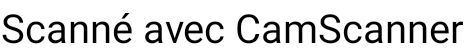
\includegraphics[width=0.7\textwidth]{images/mpm/mpm-012-000.png}
\captionof{figure}{\small Collision élastique unidimensionnelle : conservation de la quantité de mouvement et de l'énergie cinétique.}
\end{center}
\begin{center}
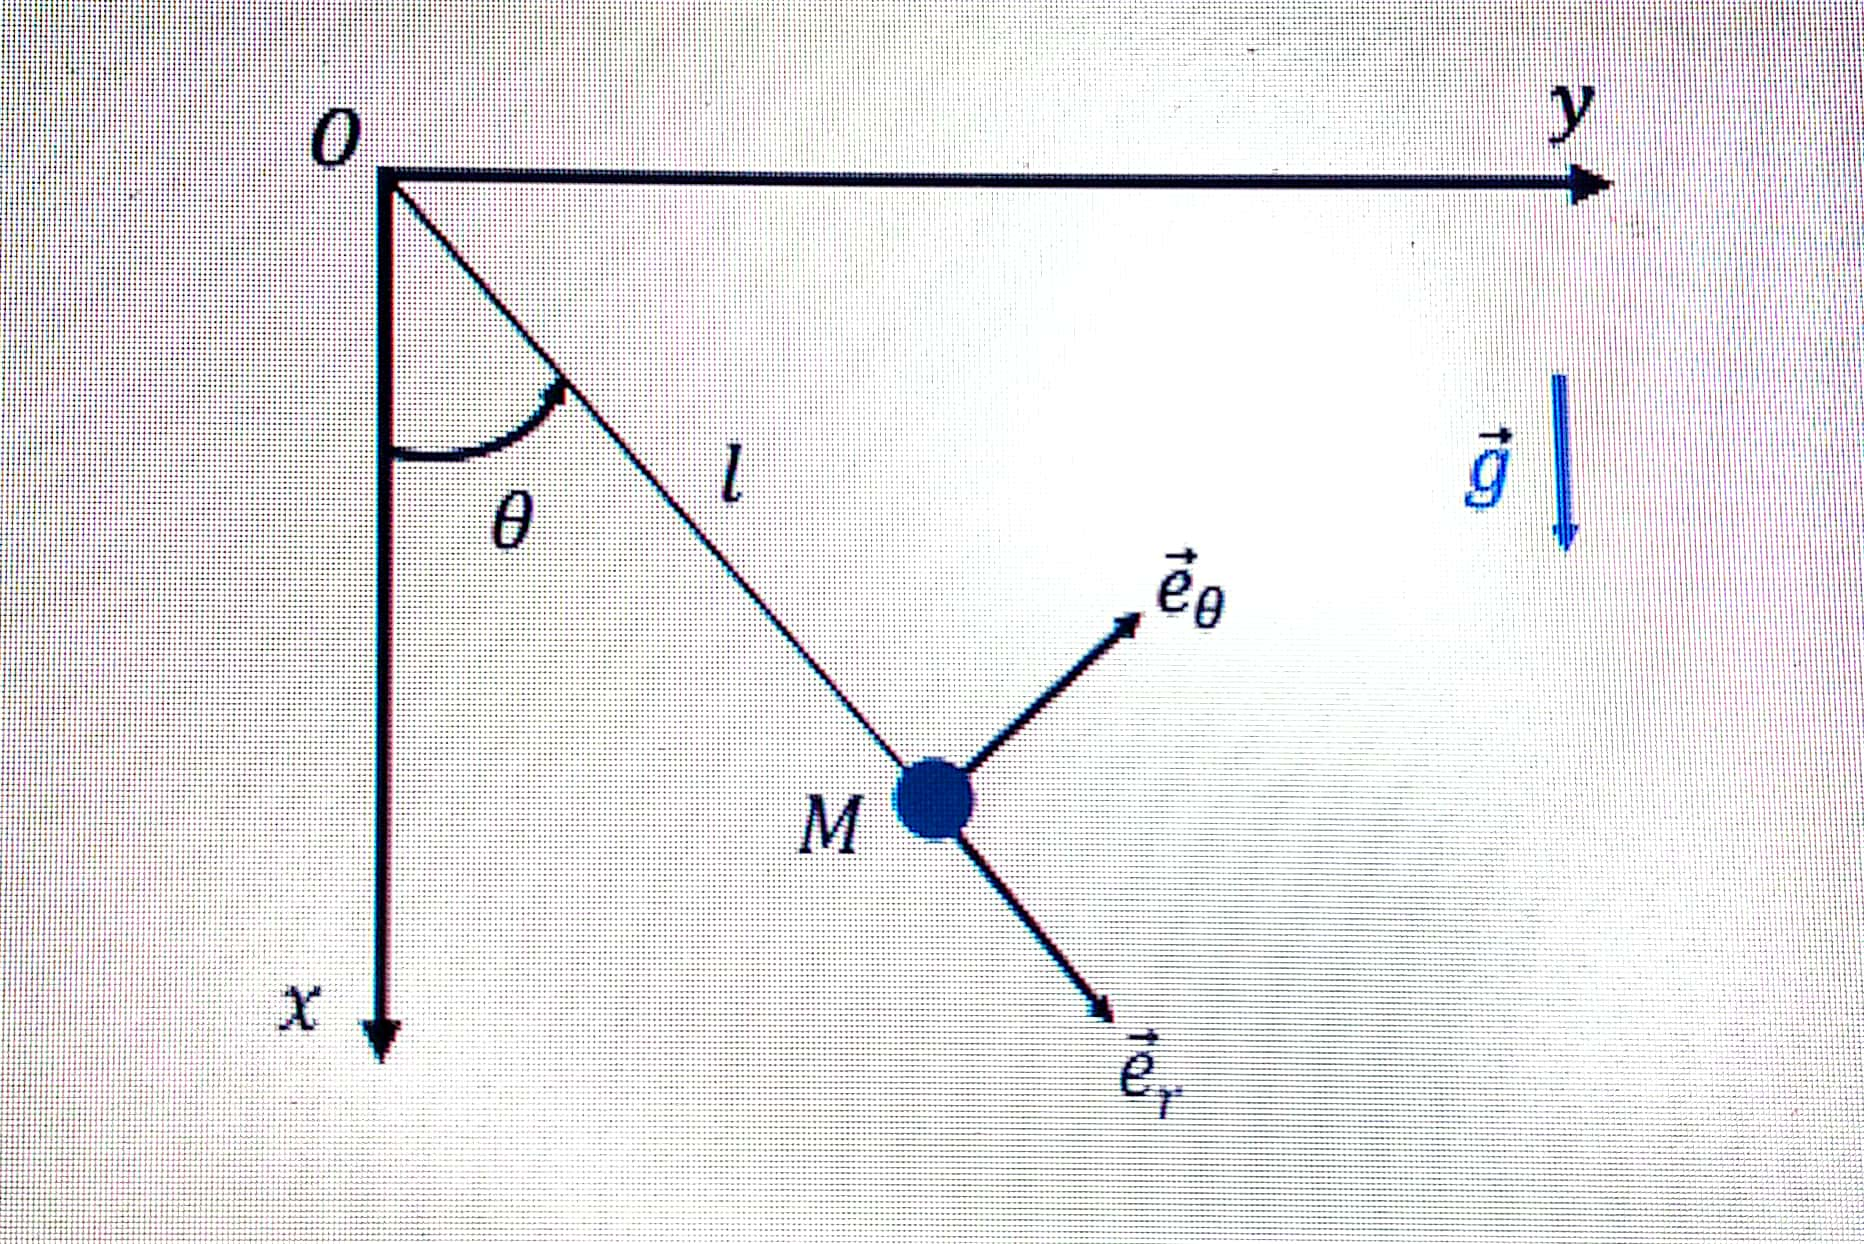
\includegraphics[width=0.55\textwidth]{images/mpm/mpm-012-001.png}
\captionof{figure}{\small Bilan énergétique avant/après choc : l'énergie cinétique est intégralement transférée entre les deux billes.}
\end{center}
\end{boitecorrige}

\subsection*{Exercice 10 - Satellite géostationnaire et troisième loi de Kepler \niveau{\moyen}}

\newpage
\begin{boiteexercice}
Un satellite géostationnaire orbite au-dessus de l'équateur à l'altitude $h = \qty{35800}{km}$.
\begin{enumerate}
  \item Calculer le rayon orbital $r = R_T + h$ avec $R_T = \qty{6371}{km}$.
  \item Calculer la vitesse orbitale $v = \sqrt{GM/r}$ avec $GM = \qty{3.98e14}{m^3.s^{-2}}$.
  \item Calculer la période $T = 2\pi r / v$ et vérifier qu'elle vaut environ $\qty{86400}{s} = \qty{24}{h}$.
  \item Vérifier la troisième loi de Kepler pour ce satellite et le satellite à $h = \qty{400}{km}$ (Exercice 4, $T \approx \qty{5573}{s}$).
\end{enumerate}
\end{boiteexercice}

\begin{boitecorrige}
\textbf{1.} Rayon orbital :
\[
r = R_T + h = (6371 + 35800)\times10^3 = 42171\times10^3 \approx \qty{4.217e7}{m}
\]

\textbf{2.} Vitesse orbitale :
\[
v = \sqrt{\frac{GM}{r}} = \sqrt{\frac{3{,}98\times10^{14}}{4{,}217\times10^7}} = \sqrt{9{,}437\times10^6} \approx \qty{3072}{m.s^{-1}}
\]

\textbf{3.} Période de révolution :
\[
T = \frac{2\pi r}{v} = \frac{2\pi\times4{,}217\times10^7}{3072} \approx \frac{2{,}649\times10^8}{3072} \approx \qty{86232}{s} \approx \qty{23.95}{h}
\]
Ce résultat est très proche de $\qty{86400}{s} = \qty{24}{h}$, ce qui justifie le caractère géostationnaire de cet orbite.
\end{boitecorrige}

\begin{center}
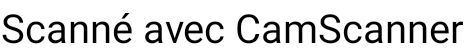
\includegraphics[width=0.85\textwidth]{images/mpm/mpm-014-002.png}
\captionof{figure}{\small Orbite géostationnaire : le satellite survole toujours le même point de l'équateur terrestre.}
\end{center}

\begin{boitecorrige}
\textbf{4.} La troisième loi de Kepler prédit $T^2/r^3 = 4\pi^2/(GM) = \text{cste}$.

Pour l'ISS ($r_1 = 6{,}8\times10^6\,\text{m}$, $T_1 = 5573\,\text{s}$) :
\[
\frac{T_1^2}{r_1^3} = \frac{(5573)^2}{(6{,}8\times10^6)^3} = \frac{3{,}106\times10^7}{3{,}144\times10^{20}} \approx 9{,}88\times10^{-14}
\]
Pour le satellite géostationnaire ($r_2 \approx 4{,}217\times10^7\,\text{m}$, $T_2 \approx 86232\,\text{s}$) :
\[
\frac{T_2^2}{r_2^3} = \frac{(86232)^2}{(4{,}217\times10^7)^3} = \frac{7{,}436\times10^9}{7{,}502\times10^{22}} \approx 9{,}91\times10^{-14}
\]
Les deux valeurs sont bien égales : la troisième loi est vérifiée.
\end{boitecorrige}

\begin{center}
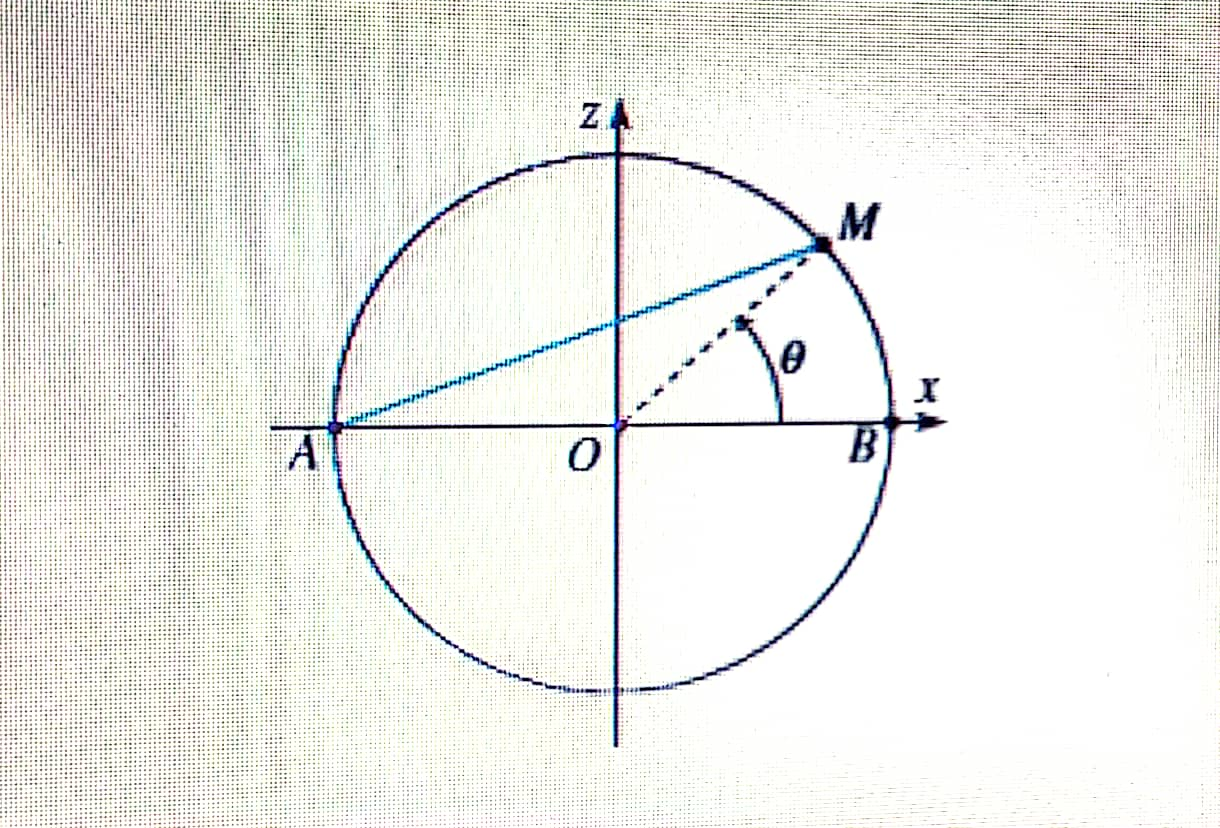
\includegraphics[width=0.55\textwidth]{images/mpm/mpm-014-003.png}
\captionof{figure}{\small Vérification graphique de la troisième loi de Kepler : $T^2$ en fonction de $r^3$ est une droite passant par l'origine.}
\end{center}

\subsection*{Exercice 11 - Théorème travail-énergie \niveau{\moyen}}

\begin{boiteexercice}
Un bloc de masse $m = \qty{10}{kg}$ est initialement au repos sur une surface horizontale. Une force horizontale $F = \qty{80}{N}$ lui est appliquée sur une distance $d = \qty{5}{m}$. Le coefficient de frottement cinétique entre le bloc et la surface est $\mu_k = 0{,}25$.
\begin{enumerate}
  \item Calculer le travail $W_F$ de la force $F$.
  \item Calculer le travail $W_{frot}$ des forces de frottement.
  \item Appliquer le théorème travail-énergie pour calculer la variation d'énergie cinétique $\Delta E_c = W_F + W_{frot}$.
  \item En déduire la vitesse finale $v_f$.
\end{enumerate}
\textbf{Donnée :} $g = \qty{9.81}{m.s^{-2}}$.
\end{boiteexercice}

\begin{boitecorrige}
\textbf{1.} Travail de la force $F$ :
\[
W_F = F\cdot d = 80\times5 = \qty{400}{J}
\]

\textbf{2.} La réaction normale est $N = mg = 10\times9{,}81 = \qty{98.1}{N}$.

La force de frottement cinétique est $f_k = \mu_k N = 0{,}25\times98{,}1 = \qty{24.525}{N}$.

Son travail (force opposée au déplacement) :
\[
W_{frot} = -f_k\cdot d = -24{,}525\times5 = \qty{-122.6}{J}
\]

\textbf{3.} Par le théorème travail-énergie :
\[
\Delta E_c = W_{total} = W_F + W_{frot} = 400 + (-122{,}6) = \qty{277.4}{J}
\]

\textbf{4.} Avec $v_0 = 0$, $E_{c,i} = 0$ :
\[
\frac{1}{2}mv_f^2 = \Delta E_c = \qty{277.4}{J}
\]
\[
v_f = \sqrt{\frac{2\times277{,}4}{10}} = \sqrt{55{,}48} \approx \qty{7.45}{m.s^{-1}}
\]
\end{boitecorrige}

\subsection*{Exercice 12 - Oscillateur harmonique amorti \niveau{\difficile}}

\newpage
\begin{boiteexercice}
Un oscillateur harmonique amorti obéit à l'équation :
\[
m\ddot{x} + b\dot{x} + kx = 0
\]
avec $m = \qty{1}{kg}$, $k = \qty{100}{N.m^{-1}}$, $b = \qty{4}{N.s.m^{-1}}$.
\begin{enumerate}
  \item Calculer la pulsation propre $\omega_0 = \sqrt{k/m}$ et le facteur de qualité $Q = m\omega_0/b$.
  \item Déterminer le régime d'amortissement (sous-amorti, critique ou sur-amorti) en comparant $b$ à $b_c = 2\sqrt{km}$.
  \item Donner la solution générale $x(t) = A\,e^{-bt/(2m)}\cos(\omega t + \varphi)$ et calculer $\omega = \sqrt{\omega_0^2 - (b/2m)^2}$.
  \item Avec les conditions initiales $x(0) = \qty{0.1}{m}$ et $\dot{x}(0) = 0$, déterminer $A$ et $\varphi$.
\end{enumerate}
\end{boiteexercice}

\begin{boitecorrige}
\textbf{1.} Pulsation propre et facteur de qualité :
\[
\omega_0 = \sqrt{\frac{k}{m}} = \sqrt{\frac{100}{1}} = \qty{10}{rad.s^{-1}}
\]
\[
Q = \frac{m\omega_0}{b} = \frac{1\times10}{4} = 2{,}5
\]

\textbf{2.} L'amortissement critique correspond à $b_c = 2\sqrt{km} = 2\sqrt{100\times1} = \qty{20}{N.s.m^{-1}}$.

Ici $b = \qty{4}{N.s.m^{-1}} < b_c = \qty{20}{N.s.m^{-1}}$, donc on est en régime \textbf{sous-amorti} ($Q > 1/2$).

\textbf{3.} En régime sous-amorti, la solution est :
\[
x(t) = A\,e^{-bt/(2m)}\cos(\omega t + \varphi)
\]
avec
\[
\omega = \sqrt{\omega_0^2 - \left(\frac{b}{2m}\right)^2} = \sqrt{100 - \left(\frac{4}{2}\right)^2} = \sqrt{100 - 4} = \sqrt{96} \approx \qty{9.80}{rad.s^{-1}}
\]
Le coefficient d'amortissement est $\gamma = b/(2m) = 4/(2\times1) = \qty{2}{s^{-1}}$.
\end{boitecorrige}

\begin{center}
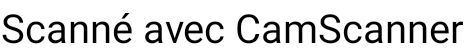
\includegraphics[width=0.85\textwidth]{images/mpm/mpm-015-004.png}
\captionof{figure}{\small Régime sous-amorti : oscillations de pulsation $\omega$ amorties exponentiellement par $e^{-\gamma t}$.}
\end{center}

\clearpage
\begin{boitecorrige}
\textbf{4.} Conditions initiales $x(0) = 0{,}1\,\text{m}$ et $\dot{x}(0) = 0$ :
\[
x(0) = A\cos\varphi = 0{,}1
\]
\[
\dot{x}(0) = A\left(-\gamma\cos\varphi - \omega\sin\varphi\right) = 0 \quad \Rightarrow \quad \tan\varphi = -\frac{\gamma}{\omega} = -\frac{2}{9{,}80} \approx -0{,}204
\]
\[
\varphi = \arctan(-0{,}204) \approx -0{,}202\,\text{rad}, \qquad A = \frac{0{,}1}{\cos\varphi} \approx \frac{0{,}1}{0{,}979} \approx \qty{0.102}{m}
\]
La solution est donc : $x(t) \approx 0{,}102\,e^{-2t}\cos(9{,}80\,t - 0{,}202)\,[\text{m}]$.
\end{boitecorrige}

\begin{center}
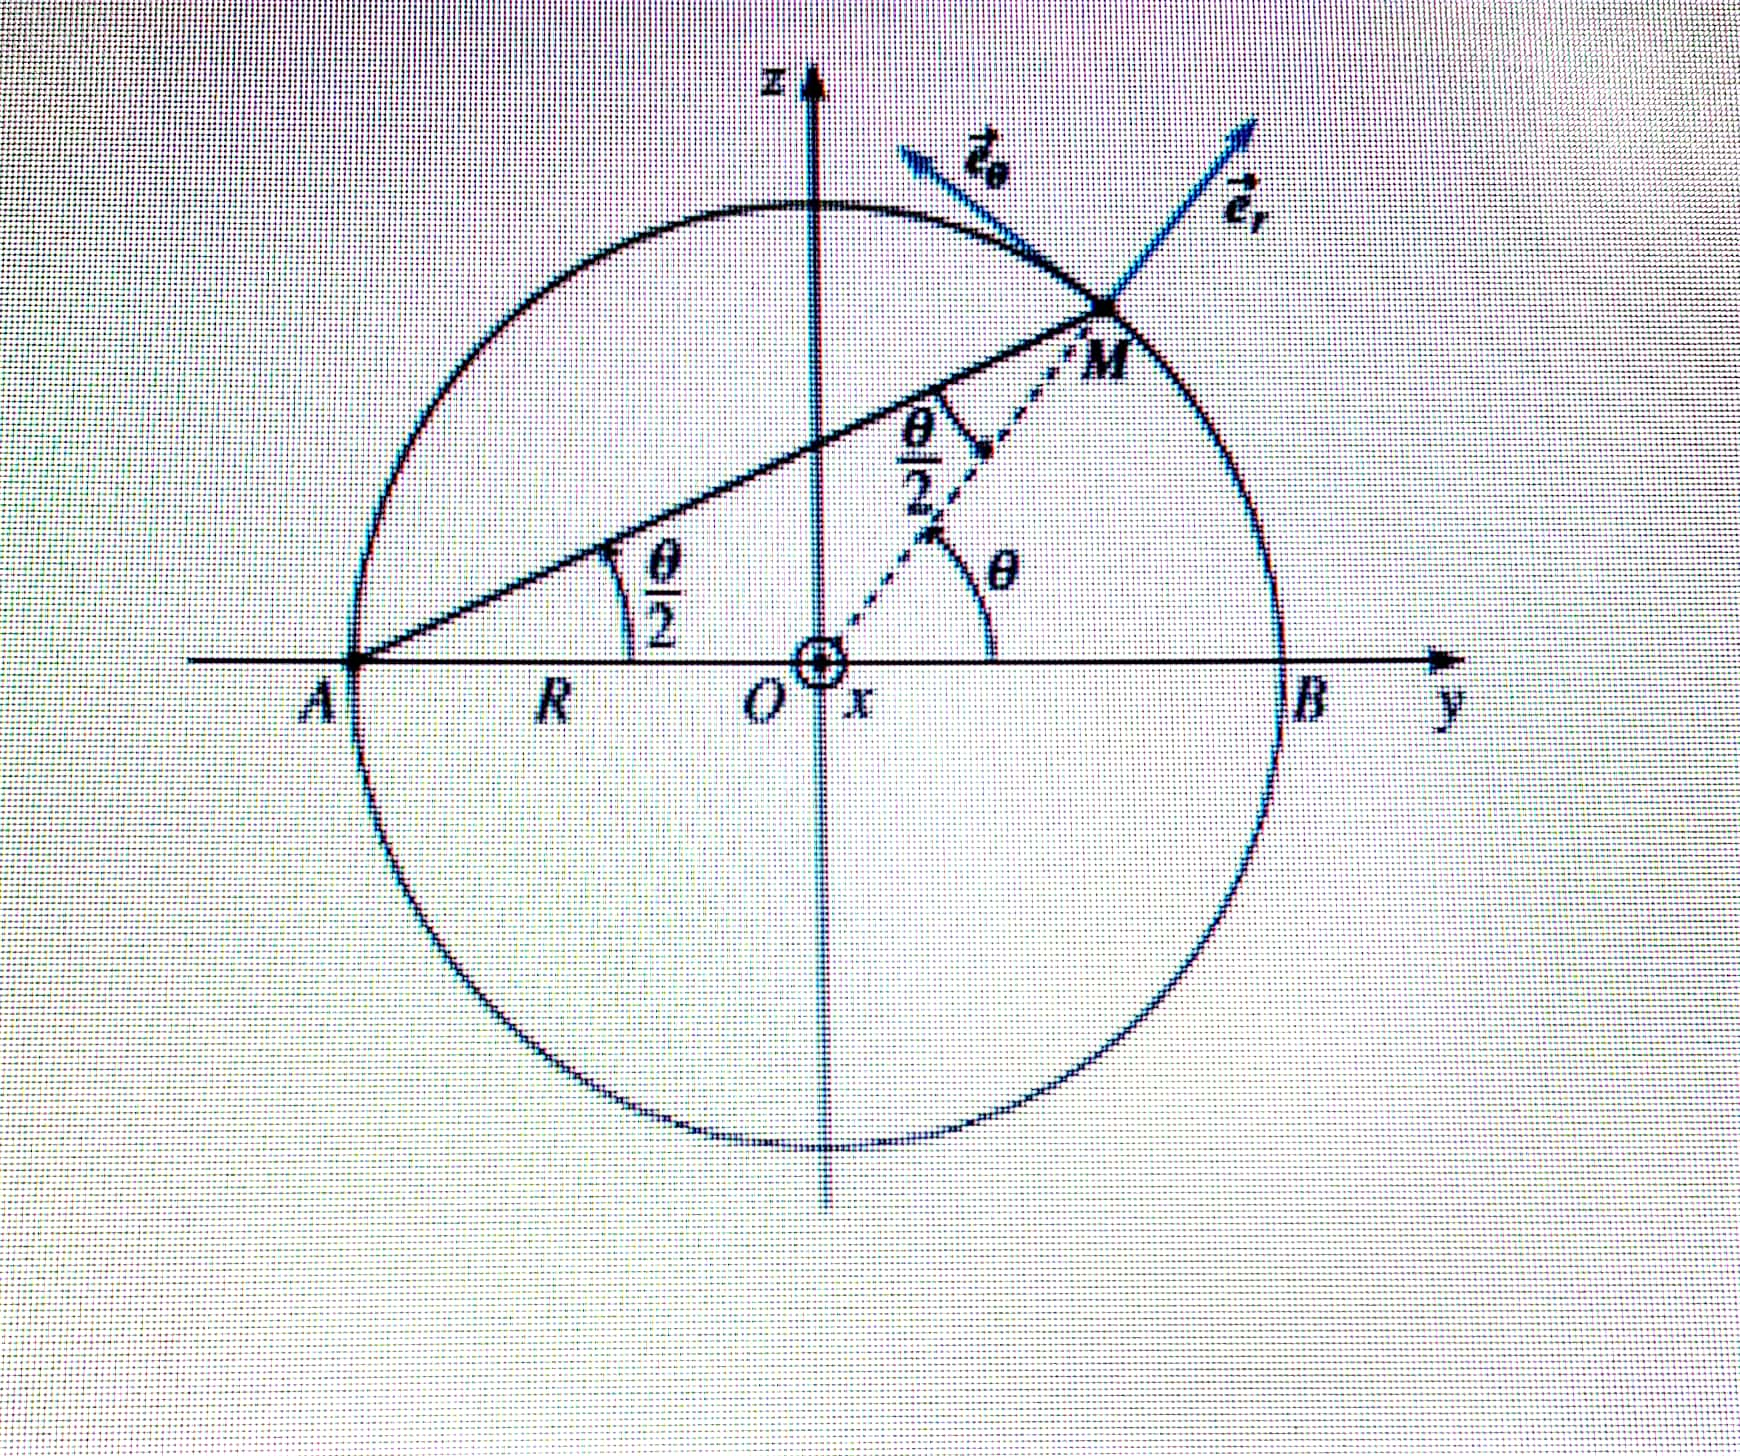
\includegraphics[width=0.55\textwidth]{images/mpm/mpm-015-005.png}
\captionof{figure}{\small Détermination graphique de $A$ et $\varphi$ à partir des conditions initiales.}
\end{center}

\subsection*{Exercice 13 - Chute verticale avec résistance de l'air \niveau{\difficile}}

\begin{boiteexercice}
Un parachutiste de masse totale $m = \qty{80}{kg}$ tombe en chute libre. La force de résistance de l'air est $f = -bv$ avec $b = \qty{10}{kg.s^{-1}}$. Il commence avec une vitesse nulle ($v(0)=0$).
\begin{enumerate}
  \item Écrire l'équation différentielle du mouvement (axe $z$ orienté vers le bas) :
  $m\dot{v} = mg - bv$.
  \item Résoudre cette équation et trouver $v(t)$.
  \item Déterminer la vitesse limite $v_\infty = mg/b$ et calculer sa valeur numérique.
  \item Calculer le temps $t^* = m/b$ au bout duquel le parachutiste atteint $63\,\%$ de la vitesse limite.
  \item Déterminer $z(t)$ (position), en prenant $z(0) = 0$.
\end{enumerate}
\textbf{Donnée :} $g = \qty{9.81}{m.s^{-2}}$.
\end{boiteexercice}

\begin{boitecorrige}
\textbf{1.} Bilan des forces sur l'axe vertical descendant : poids $mg$ (vers le bas) et frottement $-bv$ (vers le haut si $v > 0$) :
\[
m\dot{v} = mg - bv
\]

\textbf{2.} L'équation s'écrit $\dot{v} + \frac{b}{m}v = g$. En posant $\alpha = b/m$ :
\[
\frac{\d v}{g - \alpha v} = \d t \quad \Rightarrow \quad -\frac{1}{\alpha}\ln|g - \alpha v| = t + C
\]
Avec $v(0) = 0$ : $C = -\frac{1}{\alpha}\ln g$.
\[
v(t) = \frac{g}{\alpha}\left(1 - \e^{-\alpha t}\right) = \frac{mg}{b}\left(1 - \e^{-bt/m}\right)
\]

\textbf{3.} Vitesse limite ($t \to \infty$) :
\[
v_\infty = \frac{mg}{b} = \frac{80\times9{,}81}{10} = \qty{78.5}{m.s^{-1}} \approx \qty{283}{km.h^{-1}}
\]

\textbf{4.} Temps caractéristique :
\[
t^* = \frac{m}{b} = \frac{80}{10} = \qty{8}{s}
\]
À $t = t^*$ : $v(t^*) = v_\infty(1 - \e^{-1}) \approx 0{,}632\,v_\infty = \qty{49.6}{m.s^{-1}}$.

\textbf{5.} En intégrant $v(t)$ :
\begin{align*}
z(t) &= \int_0^t v(t')\,\d t' = v_\infty\int_0^t \left(1-\e^{-t'/t^*}\right)\d t' \\
&= v_\infty\left[t + t^*\e^{-t/t^*}\right]_0^t = v_\infty\left(t + t^*\e^{-t/t^*} - t^*\right) \\
&= v_\infty\left(t - t^*\left(1 - \e^{-t/t^*}\right)\right)
\end{align*}
Soit numériquement : $z(t) = 78{,}5\left(t - 8(1-\e^{-t/8})\right)$ [m].
\end{boitecorrige}

\subsection*{Exercice 14 - Conservation de l'énergie : ressort et gravité \niveau{\moyen}}

\begin{boiteexercice}
Une masse $m = \qty{2}{kg}$ est attachée à un ressort vertical de constante de raideur $k = \qty{50}{N.m^{-1}}$ et de longueur à vide $L_0$. Le système est en position d'équilibre. On écarte la masse d'une distance $A = \qty{5}{cm}$ vers le bas et on la lâche.
\begin{enumerate}
  \item Calculer l'allongement à l'équilibre $\delta = mg/k$.
  \item En prenant comme référence de l'énergie potentielle gravitationnelle le point d'équilibre, écrire l'énergie mécanique totale $E_m = \frac{1}{2}mv^2 + \frac{1}{2}k x^2$ (où $x$ est l'écart à l'équilibre). Justifier.
  \item Calculer la vitesse maximale $v_{max}$ atteinte en $x = 0$.
  \item Calculer la pulsation des oscillations $\omega_0 = \sqrt{k/m}$ et la période $T$.
  \item À quelle position $x_1$ la vitesse vaut-elle $v_{max}/\sqrt{2}$ ?
\end{enumerate}
\textbf{Données :} $g = \qty{9.81}{m.s^{-2}}$.
\end{boiteexercice}

\begin{boitecorrige}
\textbf{1.} À l'équilibre, le ressort est allongé de :
\[
\delta = \frac{mg}{k} = \frac{2\times9{,}81}{50} = \qty{0.392}{m} \approx \qty{39.2}{cm}
\]

\textbf{2.} En notant $x$ l'écart par rapport à la position d'équilibre (positif vers le bas), les forces sur la masse sont : $mg$ (bas) et $-k(\delta+x)$ (ressort, haut). Le bilan :
\[
m\ddot{x} = mg - k(\delta+x) = mg - k\delta - kx = -kx
\]
(car $mg = k\delta$ à l'équilibre). L'énergie potentielle effective (gravité + ressort, au 2e ordre en $x$) se réduit à $\frac{1}{2}kx^2$ autour de l'équilibre. L'énergie mécanique est :
\[
E_m = \frac{1}{2}mv^2 + \frac{1}{2}kx^2 = \text{constante}
\]

\textbf{3.} À $t=0$ : $x = A = \qty{0.05}{m}$, $v = 0$, donc $E_m = \frac{1}{2}kA^2$.
En $x = 0$ : $\frac{1}{2}mv_{max}^2 = \frac{1}{2}kA^2$.
\[
v_{max} = A\sqrt{\frac{k}{m}} = 0{,}05\times\sqrt{\frac{50}{2}} = 0{,}05\times5 = \qty{0.25}{m.s^{-1}}
\]

\textbf{4.} Pulsation et période :
\[
\omega_0 = \sqrt{\frac{k}{m}} = \sqrt{\frac{50}{2}} = \qty{5}{rad.s^{-1}}, \quad T = \frac{2\pi}{\omega_0} = \frac{2\pi}{5} \approx \qty{1.26}{s}
\]

\textbf{5.} On cherche $x_1$ tel que $v = v_{max}/\sqrt{2}$ :
\[
\frac{1}{2}m\frac{v_{max}^2}{2} + \frac{1}{2}kx_1^2 = \frac{1}{2}kA^2
\]
\[
\frac{1}{2}kx_1^2 = \frac{1}{2}kA^2 - \frac{1}{4}kA^2 = \frac{1}{4}kA^2 \quad \Rightarrow \quad x_1 = \frac{A}{\sqrt{2}} = \frac{0{,}05}{\sqrt{2}} \approx \qty{3.54}{cm}
\]
\end{boitecorrige}

\subsection*{Exercice 15 - Mouvement dans un champ gravitationnel : orbite elliptique \niveau{\difficile}}

\begin{boiteexercice}
On considère un satellite de masse $m$ en orbite circulaire autour de la Terre (masse $M_T$, rayon $R_T = \qty{6371}{km}$).
\begin{enumerate}
  \item À l'altitude $h = \qty{400}{km}$ (altitude de la Station Spatiale Internationale), calculer le rayon orbital $r = R_T + h$, la vitesse orbitale $v = \sqrt{GM_T/r}$ et la période $T$.
  \item Montrer que l'énergie mécanique totale du satellite est $E = -\frac{GM_T m}{2r}$ (état lié).
  \item Calculer la vitesse de libération depuis la surface terrestre : $v_L = \sqrt{2GM_T/R_T}$.
  \item La troisième loi de Kepler : $T^2 = \frac{4\pi^2}{GM_T}\,r^3$. Vérifier avec les valeurs ci-dessus.
\end{enumerate}
\textbf{Données :} $G = \qty{6.674e-11}{N.m^2.kg^{-2}}$, $M_T = \qty{5.972e24}{kg}$, $g_0 = \qty{9.81}{m.s^{-2}}$.
\end{boiteexercice}

\begin{boitecorrige}
\textbf{1.} Rayon orbital :
\[
r = R_T + h = 6371 + 400 = \qty{6771}{km} = \qty{6.771e6}{m}
\]
Pour une orbite circulaire, la force de gravitation fournit la force centripète :
\[
\frac{GM_T m}{r^2} = \frac{mv^2}{r} \quad \Rightarrow \quad v = \sqrt{\frac{GM_T}{r}}
\]
\[
v = \sqrt{\frac{6{,}674\times10^{-11}\times5{,}972\times10^{24}}{6{,}771\times10^6}}
= \sqrt{\frac{3{,}986\times10^{14}}{6{,}771\times10^6}} = \sqrt{5{,}887\times10^7} \approx \qty{7673}{m.s^{-1}}
\]
\[
T = \frac{2\pi r}{v} = \frac{2\pi\times6{,}771\times10^6}{7673} \approx \qty{5545}{s} \approx \qty{92.4}{min}
\]

\textbf{2.} Énergie cinétique : $E_c = \frac{1}{2}mv^2 = \frac{GM_T m}{2r}$.

Énergie potentielle gravitationnelle : $E_p = -\frac{GM_T m}{r}$.

Énergie totale :
\[
E = E_c + E_p = \frac{GM_T m}{2r} - \frac{GM_T m}{r} = -\frac{GM_T m}{2r} < 0
\]
L'énergie négative confirme que le satellite est lié (orbite fermée).

\textbf{3.} Vitesse de libération (énergie totale nulle depuis la surface) :
\[
E = \frac{1}{2}mv_L^2 - \frac{GM_T m}{R_T} = 0 \quad \Rightarrow \quad v_L = \sqrt{\frac{2GM_T}{R_T}}
\]
\[
v_L = \sqrt{\frac{2\times6{,}674\times10^{-11}\times5{,}972\times10^{24}}{6{,}371\times10^6}}
= \sqrt{1{,}252\times10^8} \approx \qty{11.19}{km.s^{-1}}
\]

\textbf{4.} Vérification de la 3e loi de Kepler :
\[
T^2 = \frac{4\pi^2}{GM_T}r^3 = \frac{4\pi^2}{3{,}986\times10^{14}}\times(6{,}771\times10^6)^3
\]
\[
= \frac{39{,}48}{3{,}986\times10^{14}}\times3{,}103\times10^{20} = \frac{39{,}48\times3{,}103\times10^{20}}{3{,}986\times10^{14}} \approx 3{,}073\times10^7
\]
\[
T = \sqrt{3{,}073\times10^7} \approx \qty{5543}{s}
\]
Résultat en accord avec le calcul direct : $T \approx \qty{5545}{s}$.

\begin{center}
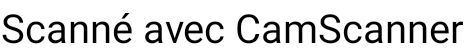
\includegraphics[width=0.7\textwidth]{images/mpm/mpm-027-006.png}
\captionof{figure}{\small Orbite circulaire autour de la Terre : équilibre entre attraction gravitationnelle et force centripète.}
\end{center}
\begin{center}
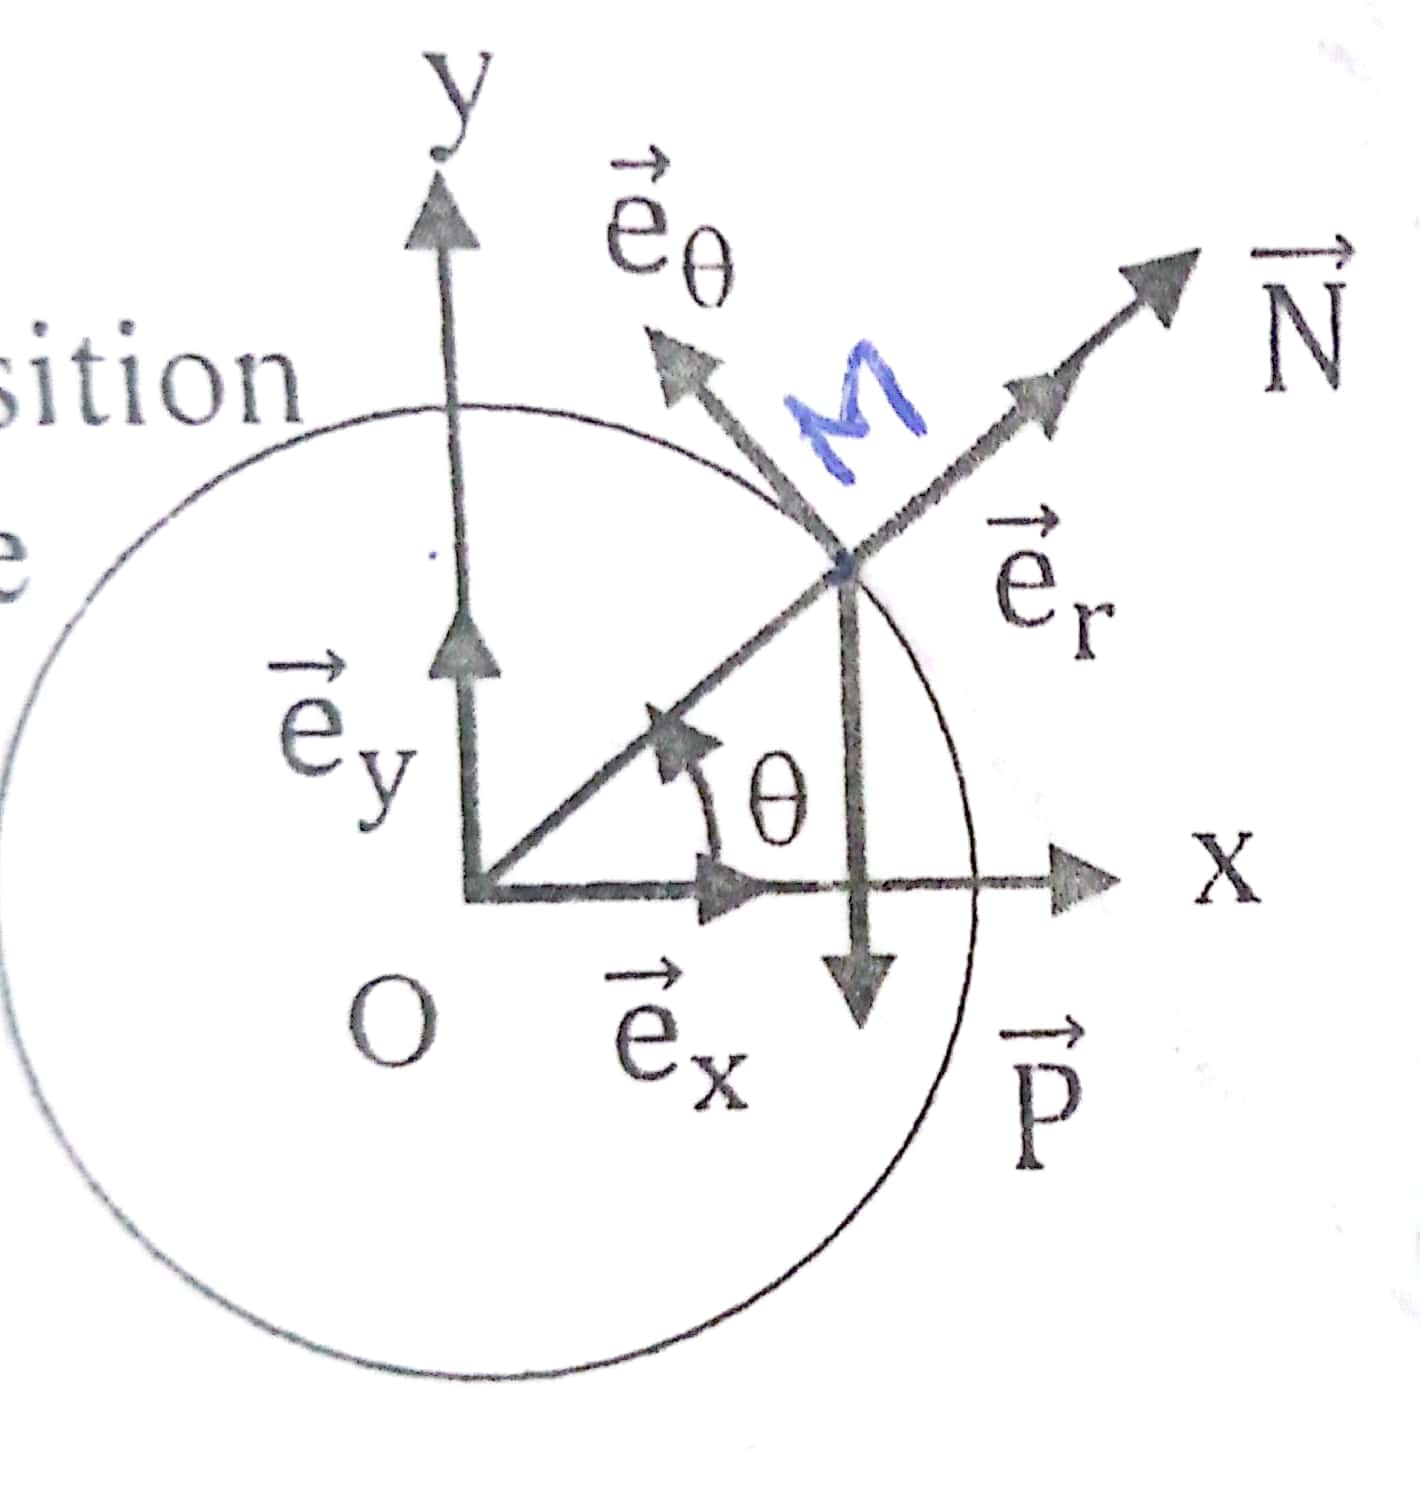
\includegraphics[width=0.55\textwidth]{images/mpm/mpm-027-007.png}
\captionof{figure}{\small Vitesse de libération et orbite de libération : $v_L = \sqrt{2GM_T/R_T}$.}
\end{center}
\end{boitecorrige}


\subsection*{Exercice 16 - Projectile avec frottement visqueux (2D) \niveau{\moyen}}

\begin{boiteexercice}
Un projectile de masse $m$ est lancé avec une vitesse initiale $v_0$ à un angle $\theta$ par rapport à l'horizontale. L'air exerce un frottement visqueux $\vec{f} = -k\vec{v}$ ($k > 0$).

\begin{enumerate}
  \item Écrire les équations du mouvement (PFD) selon les axes $x$ (horizontal) et $y$ (vertical, positif vers le haut) :
  \[
  m\dot{v}_x = -kv_x, \qquad m\dot{v}_y = -mg - kv_y
  \]
  \item Résoudre ces deux équations différentielles avec les conditions initiales $v_x(0) = v_0\cos\theta$ et $v_y(0) = v_0\sin\theta$. Montrer que :
  \[
  v_x(t) = v_0\cos\theta\,\e^{-kt/m}, \qquad v_y(t) = \left(v_0\sin\theta + \frac{mg}{k}\right)\e^{-kt/m} - \frac{mg}{k}
  \]
  \item En intégrant les vitesses, donner les expressions de $x(t)$ et $y(t)$ avec $x(0) = y(0) = 0$.
  \item Comparer qualitativement la portée avec et sans frottement. Dans quel sens le frottement modifie-t-il la trajectoire ?
\end{enumerate}

\textbf{Application numérique :} $m = \qty{0.5}{kg}$, $v_0 = \qty{30}{m.s^{-1}}$, $\theta = 45^\circ $, $k = \qty{0.05}{kg.s^{-1}}$, $g = \qty{9.81}{m.s^{-2}}$.
\end{boiteexercice}

\begin{boitecorrige}
\textbf{1.} En appliquant le PFD selon chaque axe, avec $\vec{f} = -k\vec{v}$ :
\[
m\ddot{x} = -k\dot{x} = -kv_x \qquad m\ddot{y} = -mg - kv_y
\]

\textbf{2. Résolution des EDO.}

\textit{Composante $x$ :} L'équation $m\dot{v}_x = -kv_x$ est homogène. On pose $\alpha = k/m$ :
\[
\dot{v}_x + \alpha v_x = 0 \quad \Rightarrow \quad v_x(t) = C_1\,\e^{-\alpha t}
\]
Avec $v_x(0) = v_0\cos\theta$ :
\[
\boxed{v_x(t) = v_0\cos\theta\,\e^{-kt/m}}
\]

\textit{Composante $y$ :} L'équation $m\dot{v}_y = -mg - kv_y$ s'écrit $\dot{v}_y + \alpha v_y = -g$. Solution particulière : $v_{y,p} = -g/\alpha = -mg/k$. Solution générale :
\[
v_y(t) = C_2\,\e^{-\alpha t} - \frac{mg}{k}
\]
Avec $v_y(0) = v_0\sin\theta$ :
\[
C_2 = v_0\sin\theta + \frac{mg}{k}
\]
\[
\boxed{v_y(t) = \left(v_0\sin\theta + \frac{mg}{k}\right)\e^{-kt/m} - \frac{mg}{k}}
\]

\textbf{3. Positions par intégration.}

\[
x(t) = \int_0^t v_x\,\d t' = \frac{mv_0\cos\theta}{k}\left(1 - \e^{-kt/m}\right)
\]

\[
y(t) = \int_0^t v_y\,\d t' = \frac{m}{k}\left(v_0\sin\theta + \frac{mg}{k}\right)\left(1 - \e^{-kt/m}\right) - \frac{mg}{k}\,t
\]

En développant et regroupant :
\[
\boxed{x(t) = \frac{mv_0\cos\theta}{k}\left(1 - \e^{-kt/m}\right)}
\]
\[
\boxed{y(t) = \left(\frac{mv_0\sin\theta}{k} + \frac{m^2 g}{k^2}\right)\left(1 - \e^{-kt/m}\right) - \frac{mg}{k}\,t}
\]

\textbf{4. Comparaison avec et sans frottement.}

Sans frottement ($k = 0$, vérifiable par développement en série de Taylor à l'ordre 1 en $k$), on retrouve les équations classiques $x = v_0\cos\theta\cdot t$, $y = v_0\sin\theta\cdot t - \frac{1}{2}gt^2$.

Avec frottement :
\begin{itemize}[nosep]
  \item La composante horizontale décélère exponentiellement : $x \to mv_0\cos\theta/k$ (limite finie), alors que sans frottement $x$ croît indéfiniment.
  \item La composante verticale tend vers la vitesse limite $-mg/k$ (chute terminale).
  \item La portée est donc \textbf{réduite} par le frottement.
  \item La trajectoire n'est plus symétrique : la descente est plus raide que la montée.
\end{itemize}

\textbf{Application numérique.}

$\alpha = k/m = 0{,}05/0{,}5 = \qty{0.1}{s^{-1}}$, $mg/k = 0{,}5\times9{,}81/0{,}05 = \qty{98.1}{m.s^{-1}}$.

Sans frottement : portée $R_0 = v_0^2\sin(2\theta)/g = 900/9{,}81 \approx \qty{91.7}{m}$.

Avec frottement, la portée est plus faible (le projectile touche le sol avant $x = \qty{91.7}{m}$).

\begin{center}
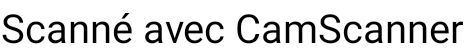
\includegraphics[width=0.7\textwidth]{images/mpm/mpm-028-008.png}
\captionof{figure}{\small Trajectoire d'un projectile avec frottement visqueux : la portée est réduite par rapport au cas sans frottement.}
\end{center}
\begin{center}
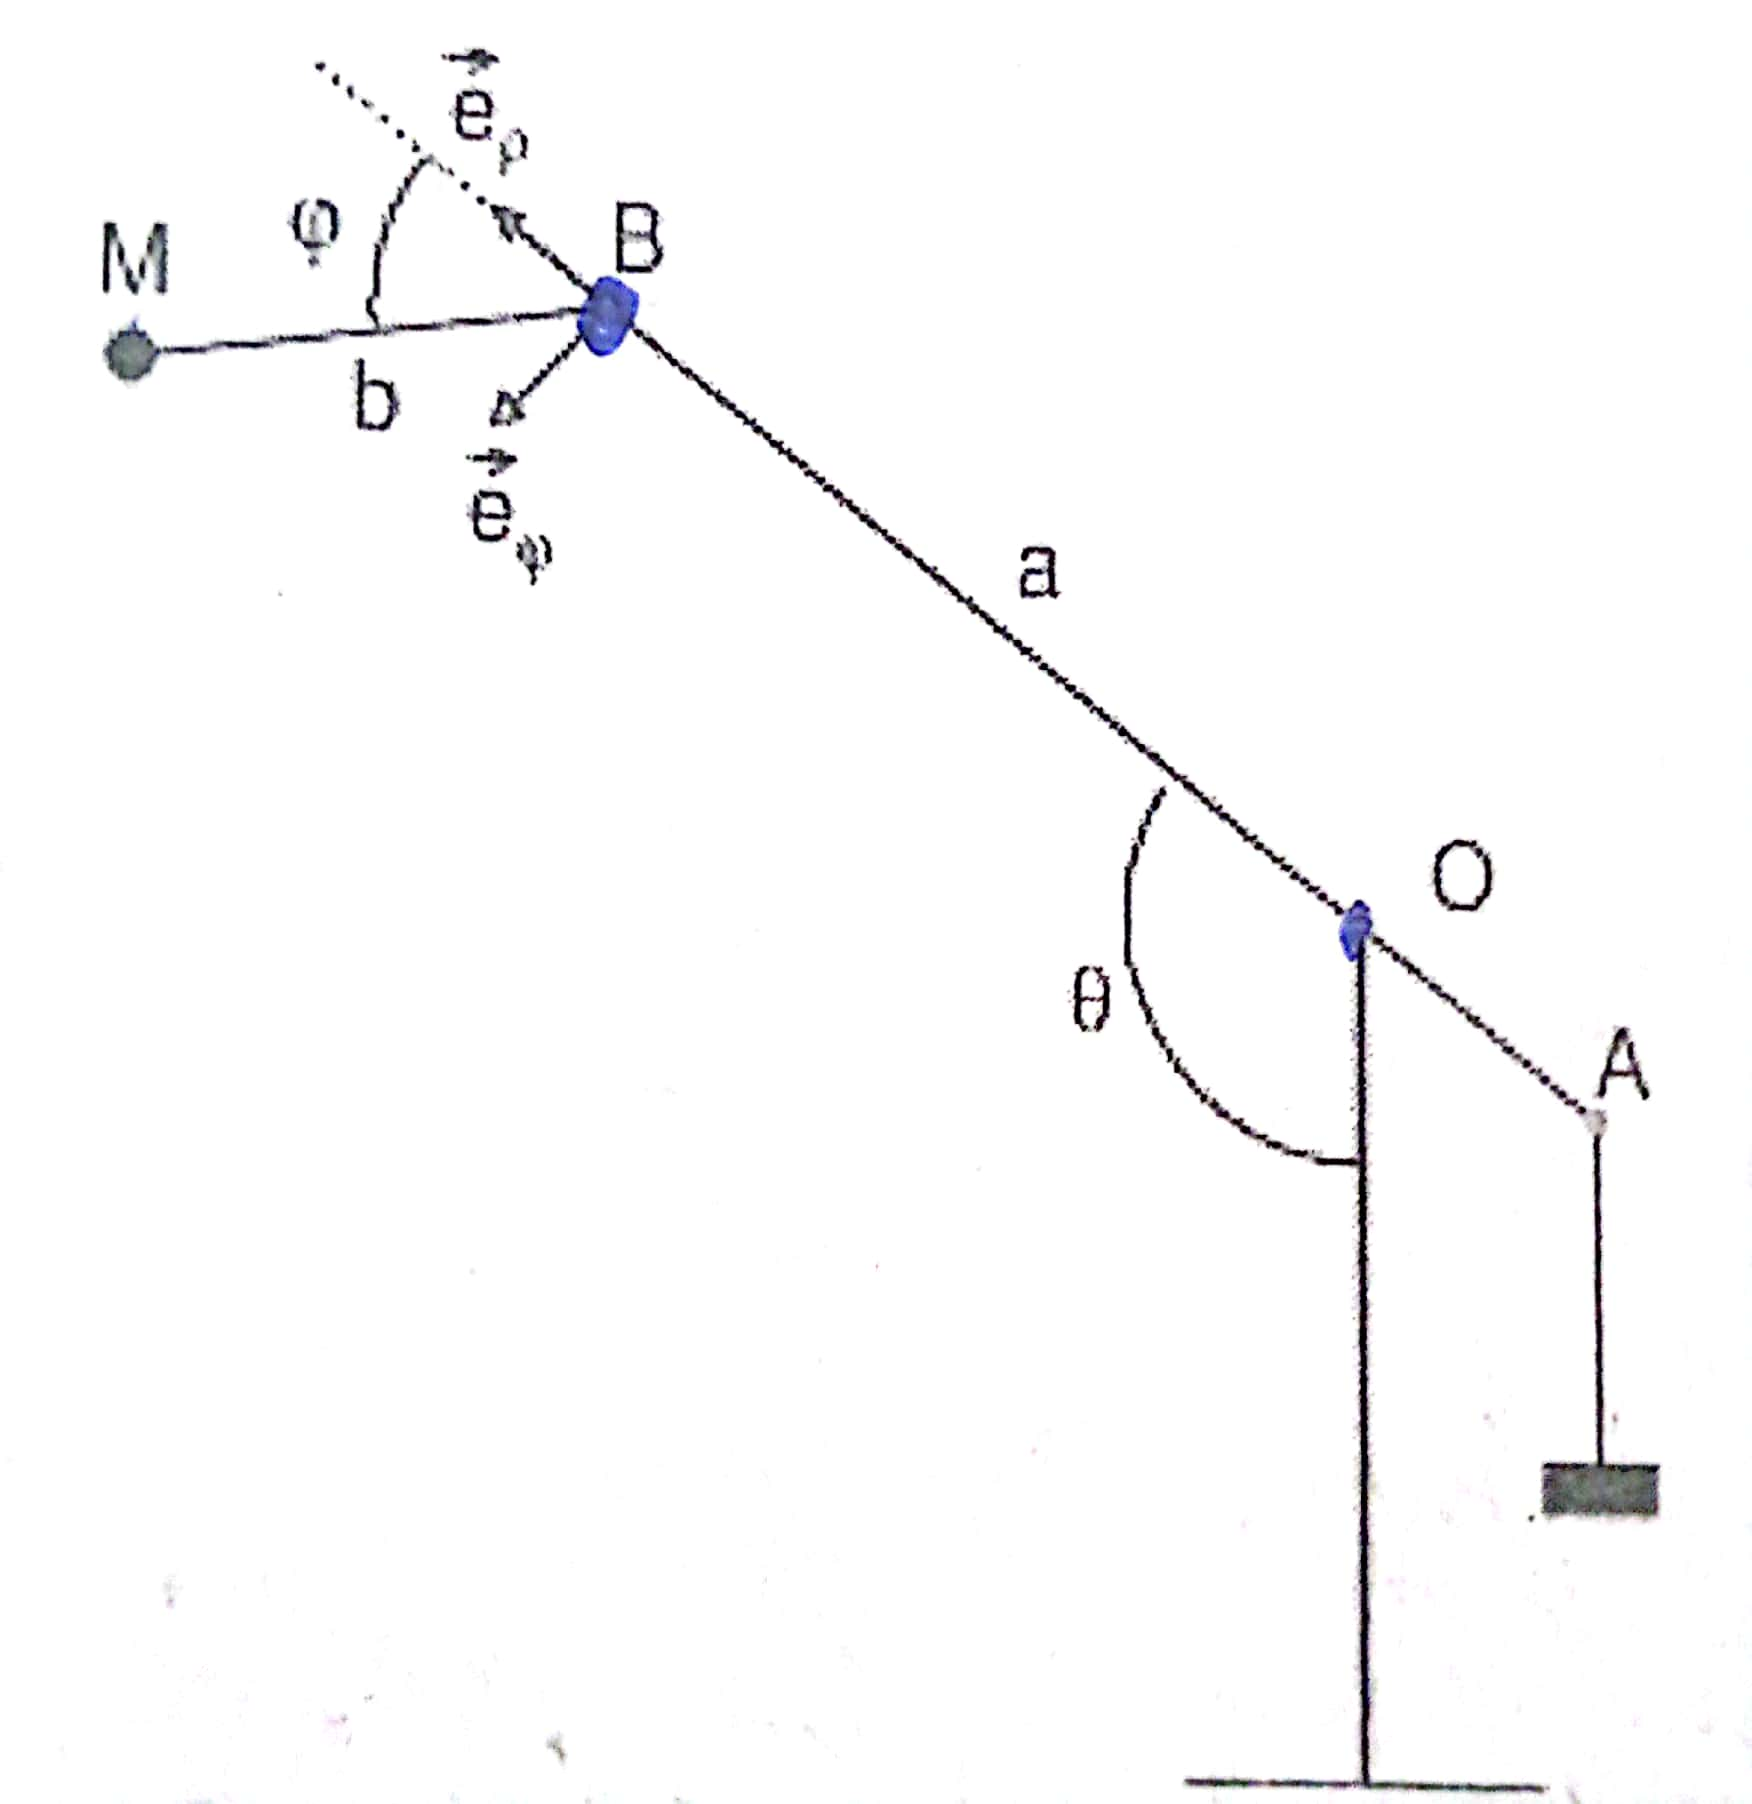
\includegraphics[width=0.55\textwidth]{images/mpm/mpm-028-009.png}
\captionof{figure}{\small Comparaison des vitesses $v_x(t)$ et $v_y(t)$ en présence de frottement fluide.}
\end{center}
\end{boitecorrige}

\subsection*{Exercice 17 - Énergie mécanique du pendule simple \niveau{\moyen}}

\begin{boiteexercice}
Un pendule simple est constitué d'une masse $m = \qty{0.2}{kg}$ suspendue à un fil de longueur $L = \qty{0.8}{m}$. On désigne par $\theta$ l'angle que fait le fil avec la verticale. Le pendule est lâché depuis $\theta_0 = 30^\circ $ sans vitesse initiale.

\begin{center}
\begin{tikzpicture}[scale=1.1]
  % Support
  \fill[gray!50] (-0.15,0) rectangle (0.15,0.15);
  \draw[gray!60, thick] (-0.9,0.15) -- (0.9,0.15);
  \fill (0,0) circle (0.055);
  % Verticale
  \draw[gray!35, dashed] (0,0) -- (0,-2.2);
  % Fil à theta0=30°
  \draw[thick] (0,0) -- ({sin(30)*1.8}, {-cos(30)*1.8});
  \shade[ball color=blue!55] ({sin(30)*1.8}, {-cos(30)*1.8}) circle (0.17);
  % Angle theta0
  \draw[->, blue!60] (0,-0.6) arc(-90:{-90+30}:0.6);
  \node[blue!70, font=\small] at (0.28, -0.52) {$\theta_0$};
  % L
  \node[left, font=\small] at (-0.12, -0.85) {$L$};
  % Position equilibre (bas)
  \shade[ball color=gray!30] (0,-1.8) circle (0.17);
  \draw[dashed, gray!50] (0,0) -- (0,-1.8);
  % Hauteur hmax
  \draw[<->, red!70] ({sin(30)*1.8+0.25}, {-cos(30)*1.8}) -- (0.25,-1.8);
  \node[red!70, right, font=\small] at (0.3, {(-cos(30)*1.8-1.8)/2}) {$h_{max}$};
  % Energie cinetique max en bas (flèche)
  \draw[->, green!60!black, very thick] (-0.25,-1.8) -- (-0.25,-1.2)
    node[left, font=\scriptsize] {$v_{max}$};
\end{tikzpicture}
\captionof{figure}{\small Pendule lâché de $\theta_0=30°$. L'énergie potentielle $E_p = mgL(1-\cos\theta_0)$ se convertit en énergie cinétique $\frac{1}{2}mv_{max}^2$ au passage par la verticale.}
\end{center}

\begin{enumerate}
  \item Écrire l'équation du mouvement (sans approximation des petits angles) :
  \[
  mL^2\ddot{\theta} = -mgL\sin\theta
  \]
  \item En utilisant la conservation de l'énergie mécanique, écrire :
  \[
  E_m = \frac{1}{2}mL^2\dot{\theta}^2 + mgL(1-\cos\theta) = \text{cste}
  \]
  Calculer la valeur de $E_m$ pour les conditions initiales données.
  \item En déduire la vitesse angulaire $\dot{\theta}$ en fonction de $\theta$. Calculer $\dot{\theta}$ quand $\theta = 0$ (passage par la verticale).
  \item En déduire la vitesse linéaire $v = L\dot{\theta}$ de la masse en bas de sa trajectoire.
  \item Linéariser l'équation du mouvement pour les petits angles. Calculer la période $T = 2\pi\sqrt{L/g}$ pour ce pendule.
  \item Quelle est la hauteur maximale $h_{max}$ atteinte par la masse au-dessus de sa position basse ?
\end{enumerate}
\textbf{Donnée :} $g = \qty{9.81}{m.s^{-2}}$.
\end{boiteexercice}

\begin{boitecorrige}
\textbf{1. Équation du mouvement.}

En appliquant le théorème du moment cinétique par rapport au point d'accrochage, avec le moment du poids :
\[
mL^2\ddot{\theta} = -mgL\sin\theta \quad \Rightarrow \quad \ddot{\theta} + \frac{g}{L}\sin\theta = 0
\]
C'est un oscillateur non linéaire.

\textbf{2. Énergie mécanique.}

L'énergie cinétique est $E_c = \frac{1}{2}mv^2 = \frac{1}{2}m(L\dot\theta)^2 = \frac{1}{2}mL^2\dot\theta^2$.

L'énergie potentielle gravitationnelle (avec origine en bas de la trajectoire, où $\theta = 0$) est :
$E_p = mgh = mgL(1 - \cos\theta)$ (la masse est à la hauteur $L - L\cos\theta = L(1-\cos\theta)$ au-dessus du point le plus bas).

\[
E_m = \frac{1}{2}mL^2\dot{\theta}^2 + mgL(1-\cos\theta)
\]

À $t = 0$ : $\theta = \theta_0 = 30^\circ $, $\dot{\theta} = 0$ :
\[
E_m = 0 + mgL(1-\cos 30^\circ ) = 0{,}2\times9{,}81\times0{,}8\times(1 - \frac{\sqrt{3}}{2})
\]
\[
E_m = 1{,}5696\times(1 - 0{,}866) = 1{,}5696\times0{,}134 \approx \qty{0.210}{J}
\]

\textbf{3. Vitesse angulaire en fonction de $\theta$.}

Par conservation de l'énergie :
\[
\frac{1}{2}mL^2\dot\theta^2 = E_m - mgL(1-\cos\theta) = mgL(\cos\theta - \cos\theta_0)
\]
\[
\boxed{\dot\theta = \pm\sqrt{\frac{2g}{L}(\cos\theta - \cos\theta_0)}}
\]

En $\theta = 0$ (verticale) :
\[
\dot\theta_{max} = \sqrt{\frac{2g}{L}(1 - \cos\theta_0)} = \sqrt{\frac{2\times9{,}81}{0{,}8}(1-\cos 30^\circ )} = \sqrt{24{,}525\times0{,}134} \approx \qty{1.814}{rad.s^{-1}}
\]

\textbf{4. Vitesse linéaire en bas.}
\[
v_{max} = L\,\dot\theta_{max} = 0{,}8\times1{,}814 \approx \qty{1.45}{m.s^{-1}}
\]

On peut aussi retrouver ce résultat par la conservation de l'énergie : $\frac{1}{2}mv_{max}^2 = E_m$, soit $v_{max} = \sqrt{2E_m/m} = \sqrt{2\times0{,}210/0{,}2} = \sqrt{2{,}1} \approx \qty{1.449}{m.s^{-1}}$.

\textbf{5. Linéarisation et période.}

Pour les petits angles, $\sin\theta \approx \theta$ (en radians). L'équation devient :
\[
\ddot{\theta} + \frac{g}{L}\theta = 0
\]
C'est un oscillateur harmonique de pulsation $\omega_0 = \sqrt{g/L}$. Période :
\[
T = \frac{2\pi}{\omega_0} = 2\pi\sqrt{\frac{L}{g}} = 2\pi\sqrt{\frac{0{,}8}{9{,}81}} = 2\pi\times0{,}285 \approx \qty{1.794}{s}
\]

Note : Cette formule est valable pour les petites oscillations. Pour $\theta_0 = 30^\circ $, la correction est de l'ordre de $1 + \frac{1}{16}\theta_0^2 \approx 1{,}03$ (soit 3\% d'écart).

\textbf{6. Hauteur maximale.}

La masse s'élève jusqu'à $\theta = \theta_0 = 30^\circ $, à la hauteur :
\[
h_{max} = L(1 - \cos\theta_0) = 0{,}8\times(1 - \cos 30^\circ ) = 0{,}8\times0{,}134 \approx \qty{0.107}{m}
\]
soit environ $\qty{10.7}{cm}$ au-dessus de la position basse.
\end{boitecorrige}

\subsection*{Exercice 18 - Pendule balistique \niveau{\difficile}}

\begin{boiteexercice}
Une balle de masse $m = \qty{10}{g}$ est tirée horizontalement à la vitesse $v_0 = \qty{400}{m.s^{-1}}$ vers une masse $M = \qty{2}{kg}$ suspendue à un fil inextensible de longueur $L = \qty{1}{m}$, initialement au repos. La balle s'incruste dans la masse (choc parfaitement inélastique).
\begin{enumerate}
  \item Calculer la vitesse $V$ de l'ensemble $(m+M)$ immédiatement après le choc (conservation de la quantité de mouvement).
  \item En utilisant la conservation de l'énergie mécanique après le choc, déterminer la hauteur maximale $h$ atteinte par le pendule.
  \item En déduire l'angle maximal $\theta_{max}$ que fait le fil avec la verticale.
  \item Calculer l'énergie cinétique pervue lors du choc et commenter.
\end{enumerate}
\textbf{Donnée :} $g = \qty{9.81}{m.s^{-2}}$.
\end{boiteexercice}

\begin{boitecorrige}
\textbf{1. Conservation de la quantité de mouvement.}

Lors du choc parfaitement inélastique, la quantité de mouvement horizontale est conservée (le système est isolé horizontalement pendant le choc très court) :
\[
mv_0 = (m+M)V \quad \Rightarrow \quad V = \frac{m}{m+M}\,v_0 = \frac{0{,}01}{2{,}01}\times400 \approx \qty{1.99}{m.s^{-1}}
\]

\textbf{2. Hauteur maximale.}

Après le choc, l'énergie mécanique du pendule se conserve (tension du fil ne travaille pas, poids est conservatif) :
\[
\frac{1}{2}(m+M)V^2 = (m+M)gh \quad \Rightarrow \quad h = \frac{V^2}{2g} = \frac{(1{,}99)^2}{2\times9{,}81} \approx \qty{0.202}{m}
\]

\textbf{3. Angle maximal.}

Géométrie du pendule : $h = L(1 - \cos\theta_{max})$, donc :
\[
\cos\theta_{max} = 1 - \frac{h}{L} = 1 - \frac{0{,}202}{1} = 0{,}798 \quad \Rightarrow \quad \theta_{max} = \arccos(0{,}798) \approx 37{,}0^\circ
\]

\textbf{4. Énergie perdue lors du choc.}

Énergie cinétique avant le choc : $E_{c,i} = \frac{1}{2}mv_0^2 = \frac{1}{2}\times0{,}01\times160000 = \qty{800}{J}$.

Énergie cinétique après le choc : $E_{c,f} = \frac{1}{2}(m+M)V^2 = \frac{1}{2}\times2{,}01\times(1{,}99)^2 \approx \qty{3.98}{J}$.

Énergie dissipée : $\Delta E = E_{c,i} - E_{c,f} \approx 800 - 3{,}98 \approx \qty{796}{J}$.

Soit un rendement $\eta = E_{c,f}/E_{c,i} \approx 0{,}5\,\%$. L'essentiel de l'énergie cinétique initiale est dissipée sous forme de chaleur (déformation) lors du choc inélastique : c'est caractéristique d'un choc parfaitement mou.
\end{boitecorrige}

\ifdefined\inMainDoc\else\end{document}\fi
